\chapter{Convolutional Models (CNNs)}\label{ch:cnn}

\glspl{CNN} represent a paradigmatic case of equivariant neural architectures, where the underlying mathematical structure dictates both their capabilities and their limitations. This chapter develops the mathematical foundations of convolutional equivariance: from its historical and empirical origins to its rigorous formalization, and the systematic extensions that arise when asking what happens when equivariance is required with respect to symmetry groups more general than translations.

We start from classical \glspl{CNN}, whose success in computer vision is mathematically explained by translation equivariance, but whose restriction to this single symmetry group also constitutes their fundamental limitation. Once these limitations are formalized and the connection with harmonic analysis is established, we systematically extend the convolution operation to increasingly general symmetry groups: finite groups, compact Lie groups such as $SO(2)$ and $SO(3)$, non-compact groups such as $SE(3)$, Riemannian manifolds without global group structure, and finally fiber bundles with local gauge equivariance. Each extension broadens the class of geometric domains that the architecture can efficiently exploit.

This progression from the initial restriction toward full generality is precisely the one predicted by the unifying framework of \autoref{ch:gdl}: \glspl{CNN} were identified there as instances of the \gls{MPNN} framework over regular grids (\autoref{prop:cnn_mpnn}), and this chapter develops in depth the mathematical foundations of that connection.

\section{Classical Convolutional Neural Networks}\label{sec:cnn_clasicas}

\glspl{CNN} arise in the context of automatic pattern recognition in images. Their origin dates back to the late 1980s and early 1990s, when Yann LeCun demonstrated their potential for handwritten digit recognition~\citep{lecun1989}.

The idea of convolutional networks is born from the techniques used to detect patterns in images. The technique was relatively simple: it consisted of a convolution with a kernel that detected a specific pattern in the image. For example, a kernel that detected horizontal, vertical, diagonal edges, etc. Mathematically, this can be translated into the following operation, where \(I\) is the image and \(K\) is the kernel:

\begin{equation}
    (I \star K)(x,y) = \sum_{u=-k}^{k}\sum_{v=-k}^{k} I(x+u, y+v)K(u,v)
    \label{eq:convolution2d}
\end{equation}

Strictly speaking, this operation is a \textit{cross-correlation}, not a convolution, since mathematical convolution uses $I(x-u, y-v)K(u,v)$ (see \autoref{def:discrete_convolution}). However, in the deep learning literature it is conventional to call it ``convolution'' because, when learning the kernel weights, the difference between convolution and cross-correlation is irrelevant: the learned kernel is simply flipped. We follow this standard convention hereafter.

A classic example illustrates the type of kernels that were designed by hand for image processing:

\begin{example}[Sobel Kernel]\label{ex:kernel_sobel}
The \textbf{Sobel kernels} detect horizontal and vertical edges through approximations of the partial derivatives:

\textbf{Horizontal Sobel} (detects vertical edges):
\[
K_x = \begin{pmatrix}
-1 & 0 & 1 \\
-2 & 0 & 2 \\
-1 & 0 & 1
\end{pmatrix}
\]

\textbf{Vertical Sobel} (detects horizontal edges):
\[
K_y = \begin{pmatrix}
-1 & -2 & -1 \\
0 & 0 & 0 \\
1 & 2 & 1
\end{pmatrix}
\]

These kernels approximate the partial derivatives $\frac{\partial I}{\partial x}$ and $\frac{\partial I}{\partial y}$ respectively, where $I(x,y)$ represents the image intensity. The gradient magnitude is computed as:
\[
|\nabla I| \approx \sqrt{(I \star K_x)^2 + (I \star K_y)^2}
\]
\end{example}

Kernels such as Sobel's exhibit revealing symmetry properties: edge detectors are antisymmetric with respect to the detection direction and sum to zero (eliminating direct-current components), while smoothing kernels are symmetric. These symmetries directly reflect the geometric transformations that each kernel detects.

The problem with using kernels was finding the specific one for each pattern to be detected; moreover, such patterns had to be simple. The solution proposed by LeCun was to use a neural network to learn the kernels. This idea can be taken a step further, not only learning kernels to detect simple patterns, but also to detect more complex patterns by applying kernels to the results of other kernels. That is, one can learn a series of kernels in the first layer of the neural network and continue adding layers of kernels on top of the previous ones to detect more complex patterns. The first layers learn simple strokes such as horizontal and vertical lines, but each subsequent layer learns more abstract concepts, such as cubes or rectangles, and so on until it is capable of recognizing complex objects such as a cat or a dog.

The explosion of convolutional networks and deep learning took place in 2012 when AlexNet won the ImageNet competition by a significant margin~\citep{alexnet}. The three necessary and relevant factors for the success of deep learning came together: a large-scale dataset, a neural network architecture that used deep learning techniques, and the processing power of \glspl{GPU}.

\begin{figure}[htbp]
    \centering
    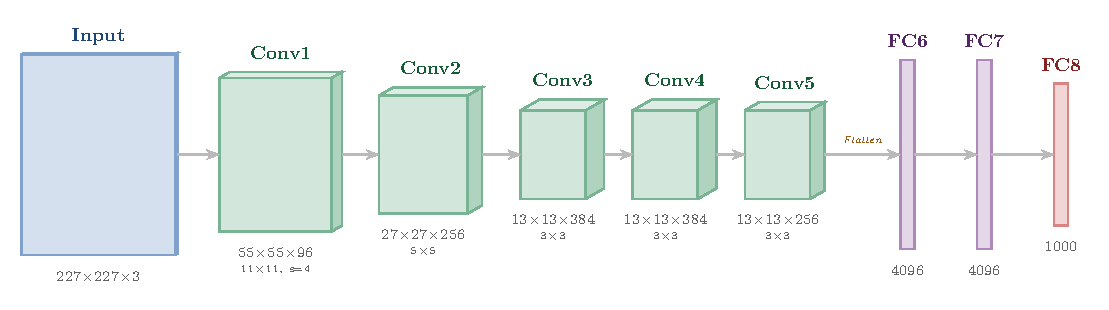
\includegraphics[width=0.95\textwidth]{images/alexnet_architecture}
    \caption[AlexNet architecture]{AlexNet architecture: a convolutional network with 8 layers (5 convolutional and 3 fully connected) that achieved a Top-5 error of 15.3\% on ImageNet ILSVRC-2012, a significant improvement over the 26.2\% of the second-best model.}
    \label{fig:alexnet}
\end{figure}

From a mathematical perspective, the central architectural principle of \glspl{CNN} is \textit{weight sharing}: the same kernels are applied at all spatial positions, which is precisely the realization of translation equivariance as an inductive bias. The local connectivity of each kernel, combined with the hierarchical composition of layers (from simple edges to abstract representations), allows the network to progressively build representations of increasing complexity. However, the restriction to the translation group also constitutes the fundamental limitation of these architectures, motivating the geometric extensions developed in the later sections of this chapter.

Convolutions can be applied not only to images, but can be extrapolated to any dimension. For example, in the case of time series, we can apply convolutions in one dimension, and in the case of 3D volumes, we can apply convolutions in three dimensions. The formulation is similar:

\begin{equation}
    (I * K)(x) = \sum_{u=-k}^{k} I(x+u)K(u)
    \label{eq:convolution1d}
\end{equation}

\begin{equation}
    (I * K)(x,y,z) = \sum_{u=-k}^{k}\sum_{v=-k}^{k}\sum_{w=-k}^{k} I(x+u, y+v, z+w)K(u,v,w)
    \label{eq:convolution3d}
\end{equation}

\subsection{Mathematical Foundations and Limitations of Classical CNNs}\label{subsec:fundamentos_limitaciones_cnn}

\subsubsection{Convolution as an Equivariant Operation}\label{subsubsec:convolucion_equivariante}

The fundamental property that makes \glspl{CNN} successful is their translation equivariance: when the input is translated, the output is translated in the same way. This property, which we will explore with a simple example, is the basis of their efficiency in image processing.

\begin{example}[Translation Equivariance in 1D]\label{ex:equivarianza_traslaciones_1d}
Consider a 1D signal $f: \mathbb{Z} \to \mathbb{R}$ and a kernel $K = [-1, 0, 1]$ (edge detector).
The translation action by $\tau \in \mathbb{Z}$ is given by $(T_\tau f)(n) = f(n-\tau)$.

Let $f = [1, 2, 1, 0, 0]$ and $\tau = 1$. Using definition~\eqref{eq:convolution1d} with zero extension outside the domain:
\begin{align}
(T_1 f) &= [0, 1, 2, 1, 0] \quad \text{(translated signal)} \\
(f * K) &= [2, 0, -2, -1, 0] \quad \text{(original convolution)} \\
((T_1 f) * K) &= [1, 2, 0, -2, -1] \quad \text{(convolution of translated signal)} \\
T_1((f * K)) &= [1, 2, 0, -2, -1] \quad \text{(translation of convolution)}
\end{align}

We observe that $((T_1 f) * K) = T_1((f * K))$, verifying the equivariance.
\end{example}

This equivariance property is fundamental to understanding both the strengths and the limitations of \glspl{CNN}. The formal concepts of equivariance and their generalization to other transformation groups are developed in detail in \autoref{ch:gdl}.

\begin{figure}[htbp]
	\centering
	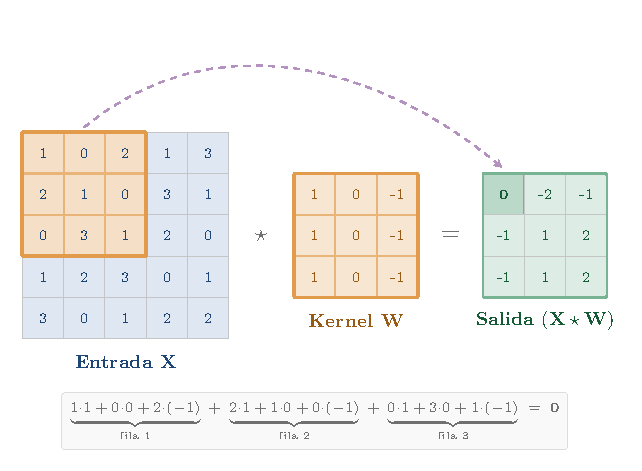
\includegraphics[width=0.85\textwidth]{images/convolution_operation}
	\caption[2D convolution operation]{2D convolution operation: a kernel $\mathbf{W}$ of size $3 \times 3$ slides over the input image $\mathbf{X}$, computing the local inner product at each position to produce the output activation map $(\mathbf{X} \star \mathbf{W})$.}
	\label{fig:convolution_operation}
\end{figure}

\begin{definition}[Discrete Convolution]\label{def:discrete_convolution}
For functions \(f, g: \mathbb{Z}^d \to \mathbb{R}\), the \textit{discrete convolution} is:
\[
(f * g)(x) = \sum_{a \in \mathbb{Z}^d} f(a)\,g(x - a)
\]
where the sum ranges over all points \(a\) of the domain \(\mathbb{Z}^d\). In practice, if \(f\) has finite support (as in a digital image), the sum reduces to the indices where \(f(a) \neq 0\).
\end{definition}

\begin{definition}[Continuous Convolution]\label{def:continuous_convolution}
For functions \(f, g: \mathbb{R}^d \to \mathbb{R}\), the \textit{continuous convolution} is:
\[
(f * g)(x) = \int_{\mathbb{R}^d} f(a)\,g(x - a) \, \mathrm{d}a
\]
where the integral is taken with respect to the Lebesgue measure over all of \(\mathbb{R}^d\), and exists when \(f, g \in L^1(\mathbb{R}^d)\) or under compact support conditions.
\end{definition}

The discrete convolution can be seen as a discretization of the continuous convolution, where the integral is approximated by a Riemann sum. In the context of digital image processing, we work with the discrete version, while in analog signals or theoretical analysis the continuous version is used.

\begin{proposition}[Algebraic Properties of Convolution]\label{prop:propiedades_convolucion}
The discrete convolution satisfies the following properties for functions
\(f, g, h: \mathbb{Z}^d \to \mathbb{R}\) with finite support:
\begin{enumerate}
    \item \textbf{Commutativity}: \(f * g = g * f\)
    \item \textbf{Associativity}: \((f * g) * h = f * (g * h)\)
    \item \textbf{Distributivity}: \(f * (g + h) = f * g + f * h\)
    \item \textbf{Identity element}: \(f * \delta = f\), where \(\delta\) is the Kronecker delta
\end{enumerate}
\end{proposition}

\begin{proof}
\textbf{(1) Commutativity.} Through the change of variable \(b = x - a\):
\begin{align}
(f * g)(x) &= \sum_{a \in \mathbb{Z}^d} f(a)\,g(x - a) = \sum_{b \in \mathbb{Z}^d} f(x - b)\,g(b) = (g * f)(x)
\end{align}

\textbf{(2) Associativity.} By direct application of the definition and reordering of summation (discrete Fubini):
\begin{align}
((f * g) * h)(x) &= \sum_{b \in \mathbb{Z}^d} (f * g)(b)\,h(x - b) = \sum_{b \in \mathbb{Z}^d} \left[\sum_{a \in \mathbb{Z}^d} f(a)\,g(b - a)\right] h(x - b) \nonumber \\
                  &= \sum_{a \in \mathbb{Z}^d} f(a) \sum_{b \in \mathbb{Z}^d} g(b - a)\,h(x - b)
\end{align}
With the change \(c = b - a\):
\begin{align}
&= \sum_{a \in \mathbb{Z}^d} f(a) \sum_{c \in \mathbb{Z}^d} g(c)\,h(x - a - c) = \sum_{a \in \mathbb{Z}^d} f(a)\,(g * h)(x - a) = (f * (g * h))(x)
\end{align}

\textbf{(3) Distributivity.} By linearity of the sum:
\begin{align}
(f * (g + h))(x) &= \sum_{a \in \mathbb{Z}^d} f(a)\,(g + h)(x - a) \nonumber \\
                  &= \sum_{a \in \mathbb{Z}^d} f(a)\,g(x - a) + \sum_{a \in \mathbb{Z}^d} f(a)\,h(x - a) = (f * g)(x) + (f * h)(x)
\end{align}

\textbf{(4) Identity element.} The Kronecker delta satisfies \(\delta(a) = 1\) if \(a = 0\) and \(\delta(a) = 0\) otherwise:
\begin{align}
(f * \delta)(x) &= \sum_{a \in \mathbb{Z}^d} f(a)\,\delta(x - a) = f(x)
\end{align}
since \(\delta(x - a) \neq 0\) only when \(a = x\).
\end{proof}

\begin{theorem}[Translation Equivariance of Convolution]\label{theorem:convolution_translation_equivariance}
The convolution operation is equivariant to the translation group \(T = \mathbb{Z}^d\):
\[
T_b(f * g) = (T_b f) * g = f * (T_b g)
\]
where \(T_b f(x) = f(x - b)\) is the translation by \(b\).
\end{theorem}

\begin{proof}
For the first equality, through the index change $a' = a - b$:
\begin{align}
[(T_b f) * g](x) &= \sum_a (T_b f)(a) g(x - a) = \sum_a f(a - b) g(x - a) \\
                  &= \sum_{a'} f(a') g(x - a' - b) = (f * g)(x - b) = [T_b(f * g)](x)
\end{align}
For the second equality:
\begin{align}
[T_b(f * g)](x) &= (f * g)(x - b) = \sum_a f(a)g((x-b) - a) \\
                 &= \sum_a f(a)g((x - a) - b) = \sum_a f(a)[T_b g](x - a) \\
                 &= [f * (T_b g)](x)
\end{align}
\end{proof}

Translation equivariance implies that the kernel weights must be shared spatially, which drastically reduces the number of parameters compared to a fully connected network. This fundamental property is generalized in \autoref{sec:group_convolutions}.

\subsubsection{Limitations of Classical CNNs}

\begin{example}[Lack of Rotational Equivariance]
Consider an image of a digit ``6'' and its $180^{\circ}$ rotation that looks like a ``9''. A standard \gls{CNN} must learn these transformations from the data through data augmentation, rather than incorporating them structurally. If $R_{90}$ denotes a $90^{\circ}$ rotation:
\[
f(R_{90}(\text{image})) \neq R_{90}(f(\text{image}))
\]
This illustrates how standard \glspl{CNN} are only equivariant to translations, not to other geometric transformations.
\end{example}

Although \glspl{CNN} have revolutionized computer vision, their design presents fundamental limitations that restrict their applicability. These limitations, which arise directly from their restriction to translation equivariance, can be classified into four main categories:

\begin{enumerate}
    \item \textbf{Symmetry limitations}: They are only equivariant to discrete translations $\mathbb{Z}^d$, requiring data augmentation for transformations such as rotations, reflections, or scalings. This is inefficient both computationally and statistically.

    \item \textbf{Topological limitations}: Designed for regular Euclidean grids, they are inadequate for data with non-trivial topologies such as graphs, point clouds, Riemannian manifolds, or simplicial complexes.

    \item \textbf{Locality limitations}: Their dependence on local structures implies that global relationships require multiple layers to be captured, limiting efficiency in domains where long-range dependencies are critical.

    \item \textbf{Receptive field limitations}: The linear growth of the receptive field with depth requires deep architectures to capture global patterns, introducing vanishing gradient problems and computational inefficiency.
\end{enumerate}

These systematic limitations have motivated the development of geometric extensions that constitute the core of this chapter. Each extension addresses specific sets of these limitations through the controlled generalization of the preserved symmetries:

\begin{itemize}
    \item \textbf{Group Convolutions} (\autoref{sec:group_convolutions}): Generalize equivariance from translations toward finite groups such as $D_4$ (rotations and reflections), addressing the symmetry limitations.
    \item \textbf{Spherical/Steerable \glspl{CNN}}: Extend equivariance to continuous groups such as $SO(2)$ and $SO(3)$, enabling the processing of spherical and three-dimensional data.
    \item \textbf{\glspl{CNN} on Manifolds} (\autoref{sec:manifold_cnns}): Overcome the topological limitations through generalization to curved surfaces and Riemannian manifolds.
    \item \textbf{Gauge Convolutions} (\autoref{sec:gauge_cnns}): Introduce equivariance to gauge transformations on fiber bundles, the most abstract generalization possible.
\end{itemize}

This systematic progression from restricted equivariance toward full generality constitutes the central narrative of the chapter and exemplifies the principles of \gls{GDL} in action.

\section{Harmonic Analysis and Spectral Convolutions}\label{sec:analisis_armonico}

While the geometric extensions of \glspl{CNN} address the limitations of symmetry, topology, and locality through the direct generalization of convolutional operations, harmonic analysis provides a dual and complementary perspective that reveals the deep mathematical structure underlying all these architectures. This section develops the theoretical framework that connects classical convolutions with their spectral generalizations, from the foundations of Fourier analysis to modern applications in irregular domains.

The spatial-spectral duality constitutes one of the most fundamental principles in applied mathematics: while convolution operations are naturally performed in the spatial domain, their algebraic structure is best understood in the frequency domain. The convolution theorem, $\mathcal{F}[f * g] = \mathcal{F}[f] \cdot \mathcal{F}[g]$, reveals that the complex convolution operation in space reduces to a simple pointwise multiplication in frequency. This perspective not only provides computational advantages through algorithms such as the \gls{FFT}, but also offers deep insights into what features neural networks learn and how more efficient architectures can be designed.

In the context of \gls{GDL}, harmonic analysis acquires fundamental importance by providing the mathematical tools needed to generalize convolutions to non-Euclidean domains. Group representation theory, developed within the framework of harmonic analysis, allows the design of convolutional layers that automatically preserve the specific symmetries of the data domain. Likewise, spectral analysis on graphs through the Laplacian provides the theoretical basis for spectral \glspl{GCN}, while wavelets offer natural hierarchical representations that align with modern deep architectures.

\subsection{Foundations of Fourier Analysis}\label{subsec:fundamentos_fourier}

Fourier analysis constitutes one of the most powerful mathematical tools for the study of periodic phenomena and frequency analysis. Its application in the context of convolutional neural networks allows a deep understanding of the spectral properties of filters and convolutional operations.

\begin{definition}[Continuous Fourier Transform]\label{def:transformada_fourier_continua}
Let $f: \mathbb{R}^d \to \mathbb{C}$ be an integrable function. The \textit{Fourier transform} of $f$ is defined as:
\begin{equation}
\mathcal{F}[f](\omega) = \hat{f}(\omega) = \int_{\mathbb{R}^d} f(x) e^{-2\pi i \omega \cdot x} dx
\end{equation}
where $\omega \in \mathbb{R}^d$ represents the frequency variable and $\omega \cdot x = \sum_{j=1}^d \omega_j x_j$ is the Euclidean dot product.
\end{definition}

\textbf{Existence Conditions.} The Fourier transform is well defined for functions in $L^1(\mathbb{R}^d)$ (absolutely integrable functions). For functions in $L^2(\mathbb{R}^d)$, the transform is defined as a mean-square limit.

\begin{definition}[Inverse Fourier Transform]\label{def:transformada_fourier_inversa}
If $\hat{f} \in L^1(\mathbb{R}^d)$, the \textit{inverse Fourier transform} is defined as:
\begin{equation}
\mathcal{F}^{-1}[\hat{f}](x) = f(x) = \int_{\mathbb{R}^d} \hat{f}(\omega) e^{2\pi i \omega \cdot x} d\omega
\end{equation}
\end{definition}

\begin{theorem}[Fourier Inversion Theorem]\label{thm:inversion_fourier}
If $f, \hat{f} \in L^1(\mathbb{R}^d)$, then:
\begin{equation}
f(x) = \mathcal{F}^{-1}[\mathcal{F}[f]](x) = \int_{\mathbb{R}^d} \hat{f}(\omega) e^{2\pi i \omega \cdot x} d\omega
\end{equation}
for almost every $x \in \mathbb{R}^d$. For the proof, see \citep[Theorem~8.26]{Folland1999}.
\end{theorem}

\begin{definition}[Convolution on $\mathbb{R}^d$]\label{def:convolucion_continua}
For functions $f, g: \mathbb{R}^d \to \mathbb{C}$, the \textit{convolution} is defined as:
\begin{equation}
(f * g)(x) = \int_{\mathbb{R}^d} f(y) g(x - y) dy = \int_{\mathbb{R}^d} f(x - y) g(y) dy
\end{equation}
when the integral converges.
\end{definition}

\subsubsection{Concrete Examples of Fourier Transforms}

The following examples illustrate the fundamental properties of the Fourier transform in contexts relevant to the analysis of CNNs.

\begin{example}[Transform of the Gaussian Function]\label{ex:fourier_gaussian}
For the Gaussian function $f(x) = e^{-\alpha x^2}$ with $\alpha > 0$:
\begin{equation}
\mathcal{F}[e^{-\alpha x^2}](\omega) = \sqrt{\frac{\pi}{\alpha}} e^{-\pi^2 \omega^2/\alpha}
\end{equation}

\textbf{Notable properties}:
\begin{itemize}
    \item The transform of a Gaussian is another Gaussian
    \item Dual localization: narrow function $\Leftrightarrow$ wide transform
    \item Minimizes the time-frequency uncertainty principle
    \item Fundamental in smoothing filters for CNNs
\end{itemize}
\end{example}

\begin{example}[Transform of the Step Function]\label{ex:fourier_step}
For the unit step function $\mathbf{1}_{[0,1]}(x)$:
\begin{equation}
\mathcal{F}[\mathbf{1}_{[0,1]}](\omega) = \frac{e^{-2\pi i \omega} - 1}{-2\pi i \omega} = \frac{\sin(\pi\omega)}{\pi\omega} e^{-\pi i \omega}
\end{equation}

\textbf{Interpretation for CNNs}:
\begin{itemize}
    \item Represents averaging filters (constant kernels)
    \item The sinc function in frequency indicates low-pass behavior
    \item Oscillations in frequency due to discontinuities in the spatial domain
\end{itemize}
\end{example}

\begin{example}[Transform of the Sinc Function]\label{ex:fourier_sinc}
For the sinc function $f(x) = \frac{\sin(\pi x)}{\pi x}$:
\begin{equation}
\mathcal{F}[\operatorname{sinc}(x)](\omega) = \mathbf{1}_{[-1/2,1/2]}(\omega)
\end{equation}

This step $\leftrightarrow$ sinc duality is fundamental:
\begin{itemize}
    \item Ideal low-pass filter in frequency $\rightarrow$ sinc response in space
    \item Impossible to implement exactly (infinite support)
    \item Inspires the design of approximate filters in spectral CNNs
\end{itemize}
\end{example}

\begin{example}[Transform of the Dirac Delta]\label{ex:fourier_delta}
For the delta distribution $\delta(x)$:
\begin{equation}
\mathcal{F}[\delta](\omega) = 1 \quad \text{and} \quad \mathcal{F}[1](\omega) = \delta(\omega)
\end{equation}

\textbf{Meaning for CNNs}:
\begin{itemize}
    \item Spatial delta = flat spectrum (all frequencies present)
    \item Spatial constant = frequency impulse (zero frequency only)
    \item Localization principle in the spectral analysis of filters
\end{itemize}
\end{example}

\textbf{Computational Implementation.} In practice, these transforms are computed through the discrete \gls{FFT}. The spectral analysis of common kernels reveals important patterns:

\textbf{Analysis process}:
\begin{enumerate}
    \item \textbf{Padding}: The kernel is extended with zeros to improve frequency resolution
    \item \textbf{2D \gls{FFT}}: The two-dimensional fast Fourier transform is computed
    \item \textbf{Spectrum centering}: fftshift is applied to center the low frequencies
    \item \textbf{Magnitude and phase analysis}: The components are separated for interpretation
\end{enumerate}

\textbf{Examples of typical kernels}:
\begin{itemize}
    \item \textbf{Sobel X}: Edge detector with high-pass response in the horizontal direction
    \item \textbf{Gaussian}: Low-pass filter with smooth and symmetric response
    \item \textbf{Laplacian}: Isotropic edge detector with high-pass response
\end{itemize}

\textbf{Connection with Wavelets.} The previous transforms motivate the use of wavelets in CNNs:
\begin{itemize}
    \item \textbf{Gaussians}: Basis for Gabor wavelets (time-frequency analysis)
    \item \textbf{Steps}: Related to Haar wavelets (edge features)
    \item \textbf{Sinc}: Foundation of Daubechies wavelets (perfect reconstruction)
\end{itemize}
The ability to analyze multiple scales simultaneously makes wavelets especially attractive for hierarchical CNN architectures.

\begin{figure}[htbp]
	\centering
	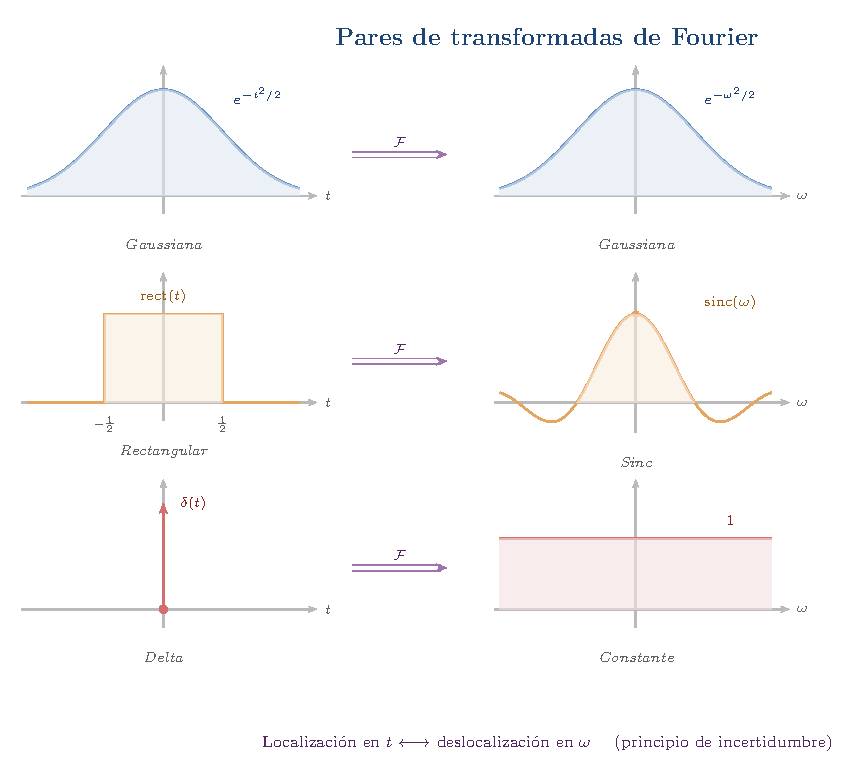
\includegraphics[width=0.85\textwidth]{images/fourier_pairs}
	\caption[Fourier transform pairs]{Fourier transform pairs: correspondence between signals in the time domain ($t$) and their representations in the frequency domain ($\omega$). The localization-delocalization duality that underlies the uncertainty principle is observed.}
	\label{fig:fourier_pairs}
\end{figure}

\subsection{Fundamental Properties of Harmonic Analysis}\label{subsec:propiedades_fundamentales}

\begin{theorem}[Convolution Theorem in the Fourier Domain]\label{thm:convolucion_fourier}
For functions \(f, g: \mathbb{R}^d \to \mathbb{C}\):
\[
\mathcal{F}[f * g] = \mathcal{F}[f] \cdot \mathcal{F}[g]
\]
where \(\mathcal{F}\) denotes the Fourier transform.
\end{theorem}

\begin{proof}
Let $f, g \in L^1(\mathbb{R}^d)$. Applying Fubini's theorem:
\begin{align}
\mathcal{F}[f * g](\omega) &= \int_{\mathbb{R}^d} (f * g)(x) e^{-2\pi i\omega \cdot x} dx \\
&= \int_{\mathbb{R}^d} \left[\int_{\mathbb{R}^d} f(y)g(x-y) \, dy\right] e^{-2\pi i\omega \cdot x} dx \\
&= \int_{\mathbb{R}^d} f(y) \left[\int_{\mathbb{R}^d} g(x-y) e^{-2\pi i\omega \cdot x} dx\right] dy \\
&= \int_{\mathbb{R}^d} f(y) e^{-2\pi i\omega \cdot y} \mathcal{F}[g](\omega) \, dy \\
&= \mathcal{F}[f](\omega) \cdot \mathcal{F}[g](\omega)
\end{align}
where in the fourth step the change of variable $z = x - y$ and the definition of $\mathcal{F}[g]$ are used.
\end{proof}

\begin{corollary}[Computational Efficiency via FFT]
The convolution can be computed in \(O(n \log n)\) using:
\[
f * g = \mathcal{F}^{-1}[\mathcal{F}[f] \cdot \mathcal{F}[g]]
\]
\end{corollary}

\begin{proof}
By the previous convolution theorem, $\mathcal{F}[f * g] = \mathcal{F}[f] \cdot \mathcal{F}[g]$, hence $f * g = \mathcal{F}^{-1}[\mathcal{F}[f] \cdot \mathcal{F}[g]]$. For discrete signals of length $n$, the \gls{FFT} computes $\mathcal{F}[f]$ and $\mathcal{F}[g]$ each in $O(n \log n)$ operations, the pointwise multiplication $\mathcal{F}[f] \cdot \mathcal{F}[g]$ requires $O(n)$ operations, and the inverse transform $\mathcal{F}^{-1}$ has the same cost $O(n \log n)$. The total cost is $O(n \log n)$, compared to the $O(n^2)$ of the direct computation of the convolution.
\end{proof}

\begin{theorem}[Plancherel Identity]\label{thm:plancherel}
For functions $f, g \in L^2(\mathbb{R}^d)$, the Fourier transform preserves the inner product:
\begin{equation}
\langle f, g \rangle_{L^2} = \langle \hat{f}, \hat{g} \rangle_{L^2}
\end{equation}
In particular, $\|\hat{f}\|_{L^2} = \|f\|_{L^2}$ (isometry). See \citep[Theorem~8.29]{Folland1999}.
\end{theorem}

\textbf{Importance in Neural Networks.} The Plancherel identity guarantees that operations in the frequency domain preserve the energy of signals, which is fundamental for the numerical stability of spectral algorithms in CNNs.

\begin{definition}[Discrete Fourier Transform (DFT)]\label{def:dft}
For a finite sequence $\{x_n\}_{n=0}^{N-1}$, the \textbf{discrete Fourier transform} is defined as:
\begin{equation}
X_k = \sum_{n=0}^{N-1} x_n e^{-2\pi i kn/N}, \quad k = 0, 1, \ldots, N-1
\end{equation}
\end{definition}

\begin{definition}[Fast Fourier Transform (FFT)]\label{def:fft}
The \gls{FFT} algorithm computes the DFT in time $O(N \log N)$ instead of $O(N^2)$ through recursive factorization:
\begin{equation}
X_k = \sum_{n=0}^{N/2-1} x_{2n} e^{-2\pi i kn/(N/2)} + e^{-2\pi i k/N} \sum_{n=0}^{N/2-1} x_{2n+1} e^{-2\pi i kn/(N/2)}
\end{equation}
\end{definition}

\begin{theorem}[Nyquist-Shannon Sampling Theorem]\label{thm:nyquist_shannon}
Let $f: \mathbb{R} \to \mathbb{C}$ be a band-limited function with $\hat{f}(\omega) = 0$ for $|\omega| > W$. Then $f$ is completely determined by its samples at intervals of $1/(2W)$:
\begin{equation}
f(t) = \sum_{n=-\infty}^{\infty} f\left(\frac{n}{2W}\right) \operatorname{sinc}(2W(t - \frac{n}{2W}))
\end{equation}
where $\operatorname{sinc}(x) = \sin(\pi x)/(\pi x)$. This fundamental result was established by \citet{Shannon1948}.
\end{theorem}

\textbf{Nyquist Frequency and Aliasing.} The Nyquist frequency $f_N = W$ is the maximum frequency that can be represented without aliasing. In CNNs, downsampling (pooling) can introduce aliasing if appropriate anti-aliasing filters are not applied.

\begin{definition}[Fourier Series]\label{def:serie_fourier}
For a periodic function $f: \mathbb{R} \to \mathbb{C}$ with period $T$, the Fourier series is expressed as:
\begin{equation}
f(t) = \sum_{n=-\infty}^{\infty} c_n e^{2\pi i n t/T}
\end{equation}
where the coefficients are $c_n = \frac{1}{T} \int_0^T f(t) e^{-2\pi i n t/T} dt$.
\end{definition}

\begin{definition}[Short-Time Fourier Transform (STFT)]\label{def:stft}
To analyze non-stationary signals, it is defined as:
\begin{equation}
\text{STFT}_f(t, \omega) = \int_{-\infty}^{\infty} f(\tau) w(\tau - t) e^{-2\pi i \omega \tau} d\tau
\end{equation}
where $w$ is a window function (typically Gaussian or Hann).
\end{definition}

\textbf{Time-Frequency Uncertainty Principle.} The STFT is subject to the uncertainty principle: $\Delta t \cdot \Delta \omega \geq \frac{1}{4\pi}$, which implies a fundamental trade-off between temporal and frequency resolution.

\subsubsection{Numerical Examples of the Convolution Theorem}

The convolution theorem is fundamental to understanding the computational efficiency of spectral CNNs. The following examples illustrate its practical application.

\begin{example}[Fast Convolution via FFT: Complexity Analysis]\label{ex:convolution_fft_complexity}
Consider the convolution of an image $f \in \mathbb{R}^{N \times N}$ with a kernel $g \in \mathbb{R}^{K \times K}$.

\textbf{Direct method}:
\begin{equation}
(f * g)[i,j] = \sum_{u=0}^{K-1} \sum_{v=0}^{K-1} f[i-u, j-v] \cdot g[u,v]
\end{equation}
Complexity: $O(N^2 K^2)$

\textbf{Spectral method}:
\begin{align}
\hat{f} &= \text{FFT2D}(f) \quad \text{[Complexity: } O(N^2 \log N)\text{]} \\
\hat{g} &= \text{FFT2D}(\text{pad}(g, N)) \quad \text{[Complexity: } O(N^2 \log N)\text{]} \\
\hat{h} &= \hat{f} \odot \hat{g} \quad \text{[Complexity: } O(N^2)\text{]} \\
h &= \text{IFFT2D}(\hat{h}) \quad \text{[Complexity: } O(N^2 \log N)\text{]}
\end{align}
Total complexity: $O(N^2 \log N)$

\textbf{Break-even point}: The spectral method is more efficient when $K > O(\log N)$.
\end{example}

\begin{example}[Practical Implementation: Fast Convolution]\label{ex:fast_convolution_implementation}
Fast convolution through the \gls{FFT} follows these algorithmic steps:

\textbf{Spectral convolution algorithm}:
\begin{enumerate}
    \item \textbf{Sizing}: Compute the optimal size as a power of 2 for \gls{FFT} efficiency
    \item \textbf{Transformation}: Apply FFT2D to both the image and the kernel with appropriate padding
    \item \textbf{Multiplication}: Element-wise product in the frequency domain
    \item \textbf{Inversion}: IFFT2D to recover the result in the spatial domain
    \item \textbf{Cropping}: Extract the valid region of the result
\end{enumerate}

\textbf{Comparative performance analysis}:
For different image and kernel sizes, typical results show:
\begin{itemize}
    \item \textbf{Small images (64$\times$64)}: Direct method more efficient for kernels $< 7 \times 7$
    \item \textbf{Medium images (256$\times$256)}: \gls{FFT} advantageous for kernels $> 5 \times 5$
    \item \textbf{Large images (512$\times$512)}: \gls{FFT} consistently faster with speedups of 2-10x
    \item \textbf{Numerical error}: Typically $< 10^{-12}$ with double precision
\end{itemize}
\end{example}

\begin{example}[Numerical Error Analysis]\label{ex:numerical_error_analysis}
The analysis of errors in \gls{FFT} convolutions reveals important patterns of numerical stability:

\textbf{Analysis methodology}:
\begin{enumerate}
    \item \textbf{Test signals}: Use random matrices with normal distribution
    \item \textbf{Reference kernel}: Discrete Laplacian as a standard test case
    \item \textbf{Comparison}: Direct convolution vs. \gls{FFT} method
    \item \textbf{Metrics}: Relative error in L2 norm
\end{enumerate}

\textbf{Observed empirical results}:
\begin{itemize}
    \item \textbf{Typical relative error}: $10^{-12}$ to $10^{-14}$ with double precision
    \item \textbf{Scalability}: The error grows logarithmically with image size
    \item \textbf{Kernel stability}: Well-conditioned kernels minimize propagation
    \item \textbf{Accumulation pattern}: Errors concentrate in high-frequency components
\end{itemize}

\textbf{Practical implications}:
The high numerical precision (error $< 10^{-12}$) makes the \gls{FFT} method practically equivalent to the direct method for most deep learning applications, where single precision ($\sim 10^{-7}$) is standard.
\end{example}

\textbf{Advanced Optimizations.} In practical implementations of spectral CNNs:

\textbf{1. Use of FFTW (Fastest Fourier Transform in the West)}:
\begin{itemize}
    \item Hardware-specific optimization (SIMD, multi-core)
    \item Automatic planning of the optimal \gls{FFT} algorithm
    \item Speedups of 2-5x over basic implementations
\end{itemize}

\textbf{2. Overlap-Add/Overlap-Save}:
For convolutions with large kernels in CNNs, block-processing techniques are used:
\begin{itemize}
    \item Divide the image into overlapping blocks
    \item FFT of small blocks (more cache-efficient)
    \item Reconstruction with overlap handling
\end{itemize}

\textbf{3. GPU Acceleration}:
\begin{itemize}
    \item cuFFT for CUDA implementations
    \item Use of shared memory to minimize transfers
    \item Batching of multiple simultaneous convolutions
\end{itemize}

\subsection{Harmonic Analysis on Groups}\label{subsec:analisis_armonico_grupos}

Harmonic analysis on groups generalizes the classical Fourier transform to more general spaces with group structure, providing the fundamental mathematical tools for geometric convolutions in neural networks.

We recall that the \textit{Haar measure} of a locally compact group $G$ is the unique Borel measure (up to a constant) invariant under left translations: $\mu(gE) = \mu(E)$ for all $g \in G$ (\autoref{def:medida_haar_gdl} of \autoref{ch:gdl}).\label{def:medida_haar}

\textbf{Existence and Uniqueness.} Haar's theorem guarantees that every Haar measure exists and is unique up to a multiplicative constant. For finite groups, the Haar measure is the counting measure.

The fundamental concepts of group representations (including the definition of representation (\autoref{def:representacion_grupo}), irreducible representations (\autoref{def:representacion_irreducible}), and the Peter-Weyl theorem (\autoref{thm:peter_weyl})) are developed in \autoref{ch:gdl}, Section~\ref{subsec:teoria_grupos_representaciones}. Here we briefly recall the specific tools of harmonic analysis that we will use for CNNs.

The \textit{character} of a representation $\rho: G \to GL(\mathbb{C}^d)$ is the function $\chi(g) = \operatorname{tr}(\rho(g))$, and the irreducible characters satisfy the orthogonality relation $\frac{1}{|G|} \sum_{g \in G} \chi_i(g) \overline{\chi_j(g)} = \delta_{ij}$. From these tools, the Fourier transform on finite groups is defined: for $f: G \to \mathbb{C}$ and an irreducible representation $\rho_i$ of dimension $d_i$,
\begin{equation}\label{eq:fourier_grupo_finito}
\hat{f}(\rho_i) = \sum_{g\in G} f(g)\rho_i(g) \in \mathbb{C}^{d_i \times d_i},
\end{equation}
with inversion $f(g) = \frac{1}{|G|} \sum_i d_i \operatorname{tr}(\hat{f}(\rho_i) \rho_i(g^{-1}))$. The fundamental result for CNNs is the \textbf{convolution theorem}: the Fourier transform converts group convolution into a matrix product,
\begin{equation}\label{eq:convolucion_fourier_grupos}
\widehat{f *_G h}(\rho_i) = \hat{f}(\rho_i) \hat{h}(\rho_i),
\end{equation}
generalizing the classical DFT result.

\begin{example}[Cyclic Group $\mathbb{Z}_n$]\label{ex:grupo_ciclico_fourier}
For the cyclic group of order $n$, the irreducible representations are one-dimensional:
\begin{equation}
\rho_k(j) = e^{-2\pi i jk/n}, \quad k = 0, 1, \ldots, n-1
\end{equation}
The Fourier transform reduces to the classical DFT:
\begin{equation}
\hat{f}(k) = \sum_{j=0}^{n-1} f(j) e^{-2\pi i jk/n}
\end{equation}
\end{example}

\begin{example}[Dihedral Group $D_n$]\label{ex:grupo_diedrico_fourier}
For the dihedral group of order $2n$ (symmetries of an $n$-gon), the representations include:
\begin{itemize}
    \item \textbf{Trivial representations}: $\rho(g) = 1$ for all $g$
    \item \textbf{Sign representations}: $\rho(r^j) = 1$, $\rho(sr^j) = -1$
    \item \textbf{Two-dimensional representations}: For rotations and reflections
\end{itemize}
\end{example}

\subsubsection{Detailed Examples of Harmonic Analysis on Finite Groups}

The following examples provide explicit computations that illustrate the practical construction of representations and Fourier transforms for groups relevant in GDL.

\begin{example}[Cyclic Group $\mathbb{Z}_4$: Explicit Computations]\label{ex:grupo_z4_detallado}
The cyclic group $\mathbb{Z}_4 = \{0, 1, 2, 3\}$ with addition modulo 4 represents $90^\circ$ rotations.

\textbf{Irreducible representations}:
The 1D representations are homomorphisms $\rho_k: \mathbb{Z}_4 \to \mathbb{C}^*$:
\begin{align}
\rho_0(j) &= 1 \quad \text{(trivial representation)} \\
\rho_1(j) &= i^j \quad \text{where } i = e^{2\pi i/4} \\
\rho_2(j) &= (-1)^j \\
\rho_3(j) &= (-i)^j
\end{align}

\textbf{Character matrix}:
\begin{equation}
\chi = \begin{bmatrix}
1 & 1 & 1 & 1 \\
1 & i & -1 & -i \\
1 & -1 & 1 & -1 \\
1 & -i & -1 & i
\end{bmatrix}
\end{equation}

\textbf{Discrete Fourier transform}:
For a function $f: \mathbb{Z}_4 \to \mathbb{C}$, $f = (f_0, f_1, f_2, f_3)^T$:
\begin{equation}
\hat{f} = \chi f = \begin{bmatrix}
f_0 + f_1 + f_2 + f_3 \\
f_0 + if_1 - f_2 - if_3 \\
f_0 - f_1 + f_2 - f_3 \\
f_0 - if_1 - f_2 + if_3
\end{bmatrix}
\end{equation}

\textbf{Application in G-CNNs}:
\begin{itemize}
    \item Each representation $\rho_k$ corresponds to a channel in convolutions equivariant to $90^\circ$ rotations
    \item The filters are expressed as linear combinations of the representations
    \item Equivariance is automatically preserved by the group structure
\end{itemize}
\end{example}

\begin{example}[Dihedral Group $D_3$: Symmetries of the Triangle]\label{ex:grupo_d3_detallado}
$D_3$ contains the 6 symmetries of the equilateral triangle: 3 rotations and 3 reflections.

\textbf{Group elements}:
\begin{itemize}
    \item $e$: identity
    \item $r, r^2$: rotations of $120^\circ, 240^\circ$
    \item $s, sr, sr^2$: reflections about the perpendicular bisectors
\end{itemize}

\textbf{Irreducible representations}:
\begin{enumerate}
    \item \textbf{Trivial} $\rho^{(1)}$: $\rho^{(1)}(g) = 1$ for all $g$
    \item \textbf{Alternating} $\rho^{(2)}$:
    \begin{align}
    \rho^{(2)}(r^k) &= 1, \quad k = 0,1,2 \\
    \rho^{(2)}(sr^k) &= -1, \quad k = 0,1,2
    \end{align}
    \item \textbf{Two-dimensional standard} $\rho^{(3)}$:
    \begin{align}
    \rho^{(3)}(e) &= \begin{bmatrix} 1 & 0 \\ 0 & 1 \end{bmatrix} \\
    \rho^{(3)}(r) &= \begin{bmatrix} -1/2 & -\sqrt{3}/2 \\ \sqrt{3}/2 & -1/2 \end{bmatrix} \\
    \rho^{(3)}(r^2) &= \begin{bmatrix} -1/2 & \sqrt{3}/2 \\ -\sqrt{3}/2 & -1/2 \end{bmatrix} \\
    \rho^{(3)}(s) &= \begin{bmatrix} 1 & 0 \\ 0 & -1 \end{bmatrix}
    \end{align}
\end{enumerate}

\textbf{Character table}:
\begin{equation}
\begin{array}{c|ccc}
 & e & r, r^2 & s, sr, sr^2 \\
\hline
\rho^{(1)} & 1 & 1 & 1 \\
\rho^{(2)} & 1 & 1 & -1 \\
\rho^{(3)} & 2 & -1 & 0
\end{array}
\end{equation}

\textbf{Computational implementation}:
The practical implementation of the dihedral group $D_3$ requires:

\textbf{Matrix representations}:
\begin{itemize}
    \item \textbf{Identity}: $2 \times 2$ identity matrix
    \item \textbf{Rotations}: Rotation matrices for $120^\circ$ and $240^\circ$
    \item \textbf{Reflections}: Combination of a basic reflection with rotations
\end{itemize}

\textbf{Fourier transform on $D_3$}:
For a function $f: D_3 \to \mathbb{C}$, the computational process involves:
\begin{enumerate}
    \item \textbf{Trivial projection}: Average of all function values
    \item \textbf{Alternating projection}: Difference between rotations and reflections
    \item \textbf{Two-dimensional projection}: A more complex linear combination
\end{enumerate}

\textbf{Analysis example}:
For the characteristic function of rotations $f(g) = 1$ if $g$ is a rotation, $f(g) = 0$ if it is a reflection:
\begin{itemize}
    \item Trivial component: $\frac{3}{6} = 0.5$
    \item Alternating component: $\frac{3-0}{6} = 0.5$
    \item 2D component: Vector with specific structure
\end{itemize}
\end{example}

\textbf{Connection with Practical G-CNNs.} The previous computations translate directly into neural network architectures:

\textbf{For $\mathbb{Z}_4$-CNNs}:
\begin{itemize}
    \item 4 filter orientations $(0^\circ, 90^\circ, 180^\circ, 270^\circ)$
    \item Each output channel corresponds to an irreducible representation
    \item The convolution is implemented as a sum over the group orbits
\end{itemize}

\textbf{For $D_3$-CNNs}:
\begin{itemize}
    \item 6 filter transformations (3 rotations $\times$ 2 reflections)
    \item Special handling of the 2D representation (coupled channels)
    \item Application in the analysis of triangular symmetries (crystallography, materials)
\end{itemize}

\textbf{Efficient implementation}:
The fast Fourier transform on finite groups is implemented through:
\begin{equation}
\text{Complexity}: O(|G|^{3/2}) \text{ vs } O(|G|^2) \text{ for the direct DFT}
\end{equation}

\begin{example}[Connection with Wavelets on Groups]\label{ex:wavelets_grupos_finitos}
Finite groups also admit wavelet analysis through appropriate mother functions.

\textbf{Mother wavelet on $\mathbb{Z}_4$}:
\begin{equation}
\psi(j) = \delta_{j,1} - \delta_{j,3} \quad \text{(difference function)}
\end{equation}

\textbf{Wavelet family}:
\begin{equation}
\psi_{k,j}(m) = \psi((m - j) \bmod 4) \cdot \omega_4^{km}
\end{equation}
where $\omega_4 = e^{2\pi i/4}$.

This construction enables multiresolution analysis in discrete spaces with rotational symmetry.
\end{example}

\begin{definition}[Fourier Transform on Compact Groups]\label{def:fourier_grupos_compactos}
For a compact group $G$ and a function $f \in L^2(G)$, the Fourier transform is defined through the Peter-Weyl theorem:
\begin{equation}
f = \sum_{\lambda \in \widehat{G}} d_\lambda \operatorname{tr}(\hat{f}(\lambda) U^\lambda)
\end{equation}
where $\widehat{G}$ indexes the irreducible representations.
\end{definition}

\subsubsection{Harmonic Analysis on SO(2) and SO(3)}

\begin{definition}[Circular Harmonics on SO(2)]\label{def:armonicos_circulares}
For the group of planar rotations $SO(2) \cong S^1$, the irreducible representations are:
\begin{equation}
U^n(\theta) = e^{in\theta}, \quad n \in \mathbb{Z}
\end{equation}
A function $f: S^1 \to \mathbb{C}$ is expanded as:
\begin{equation}
f(\theta) = \sum_{n=-\infty}^{\infty} c_n e^{in\theta}
\end{equation}
\end{definition}

\begin{definition}[Spherical Harmonics on SO(3)]\label{def:armonicos_esfericos}
For the group of three-dimensional rotations $SO(3)$, functions on the sphere $S^2$ are expanded in spherical harmonics:
\begin{equation}
f(\theta, \phi) = \sum_{l=0}^{\infty} \sum_{m=-l}^{l} c_{lm} Y_l^m(\theta, \phi)
\end{equation}
where $Y_l^m$ are the spherical harmonics of degree $l$ and order $m$.
\end{definition}

\textbf{Applications of the Peter-Weyl Theorem.} The Peter-Weyl theorem (\autoref{thm:peter_weyl}, \autoref{ch:gdl}) provides the theoretical basis for:
\begin{itemize}
    \item The channel decomposition in G-CNNs
    \item The design of equivariant filters on spheres
    \item The efficient parametrization of convolutions on Lie groups
\end{itemize}

\subsection{Spectral Analysis on Graphs}\label{subsec:analisis_espectral_grafos}

Spectral analysis on graphs extends the ideas of Fourier analysis to irregular domains, providing the mathematical foundations for spectral convolutions in neural networks on graphs. The theoretical foundations of the graph Laplacian, including definitions and spectral properties, are developed in \autoref{ch:gdl}, Section~\ref{subsec:geometria_topologica_grafos}. For the Laplacian matrix $L = D - A$ and its normalized variants, see \autoref{def:laplaciano_grafo} and \autoref{prop:propiedades_espectrales_laplaciano_grafos}.

In this section we focus on the applications of spectral analysis to the design of convolutions on graphs, assuming familiarity with the Laplacian $L$ and its normalized version $\mathcal{L} = D^{-1/2} L D^{-1/2}$.

\begin{theorem}[Spectral Theorem for the Laplacian]\label{thm:espectral_laplaciano}
Let $L$ be the Laplacian matrix of a connected graph. Then:
\begin{enumerate}
    \item The eigenvalues satisfy $0 = \lambda_0 < \lambda_1 \leq \lambda_2 \leq \cdots \leq \lambda_{n-1}$
    \item The eigenvector associated with $\lambda_0 = 0$ is $\phi_0 = \frac{1}{\sqrt{n}} \mathbf{1}$
    \item The eigenvectors $\{\phi_k\}_{k=0}^{n-1}$ form an orthonormal basis of $\mathbb{R}^n$
    \item The multiplicity of $\lambda_0$ equals the number of connected components
\end{enumerate}
For the proof, see \citep[Chapters~1--2]{Chung1997} and \autoref{prop:propiedades_espectrales_laplaciano_grafos}.
\end{theorem}

The Fourier transform on graphs (\autoref{def:transformada_fourier_grafos}, \autoref{ch:gdl}) projects signals onto the eigenvectors of the Laplacian: $\hat{f}(\lambda_k) = \langle \mathbf{f}, \phi_k \rangle$, with matrix form $\hat{f} = U^T f$. From this transform, spectral convolutions are defined:

\begin{definition}[Spectral Convolution on Graphs]\label{def:convolucion_espectral_grafos}
For a function $f: V \to \mathbb{R}$ and a spectral filter $g: \mathbb{R}_+ \to \mathbb{R}$:
\begin{equation}
(g \star f)(v_i) = \sum_{k=0}^{n-1} g(\lambda_k) \hat{f}(\lambda_k) \phi_k(v_i)
\end{equation}
In matrix form: $g \star f = \Phi g(\Lambda) \Phi^T f$, where $\Phi = [\phi_0, \ldots, \phi_{n-1}]$ and $\Lambda = \operatorname{diag}(\lambda_0, \ldots, \lambda_{n-1})$.
\end{definition}

\begin{theorem}[Frequency Interpretation]\label{thm:interpretacion_frecuencial_grafos}
The eigenvalues of the Laplacian have a frequency interpretation:
\begin{itemize}
    \item \textbf{Low frequencies} ($\lambda_k$ small): Eigenvectors vary smoothly over the graph
    \item \textbf{High frequencies} ($\lambda_k$ large): Eigenvectors oscillate rapidly between adjacent vertices
    \item \textbf{Low-pass filters}: $g(\lambda) \approx 1$ for small $\lambda$, $g(\lambda) \approx 0$ for large $\lambda$
\end{itemize}
\end{theorem}

\begin{proof}
The interpretation is justified through the Rayleigh quotient. For a signal $\mathbf{f} \in \mathbb{R}^n$ on the graph, the total variation is measured as:
\[
\mathbf{f}^T L \mathbf{f} = \sum_{(i,j) \in E} w_{ij}(f_i - f_j)^2
\]
The $k$-th eigenvector $\phi_k$ minimizes this total variation subject to orthogonality with the previous eigenvectors: $\lambda_k = \min_{\mathbf{f} \perp \phi_0, \ldots, \phi_{k-1}} \frac{\mathbf{f}^T L \mathbf{f}}{\mathbf{f}^T \mathbf{f}}$. Hence eigenvectors with small eigenvalues minimize the variation between adjacent nodes (smooth variation, low frequency), while large eigenvalues correspond to eigenvectors with high variation (rapid oscillations, high frequency).
\end{proof}

\begin{figure}[htbp]
    \centering
    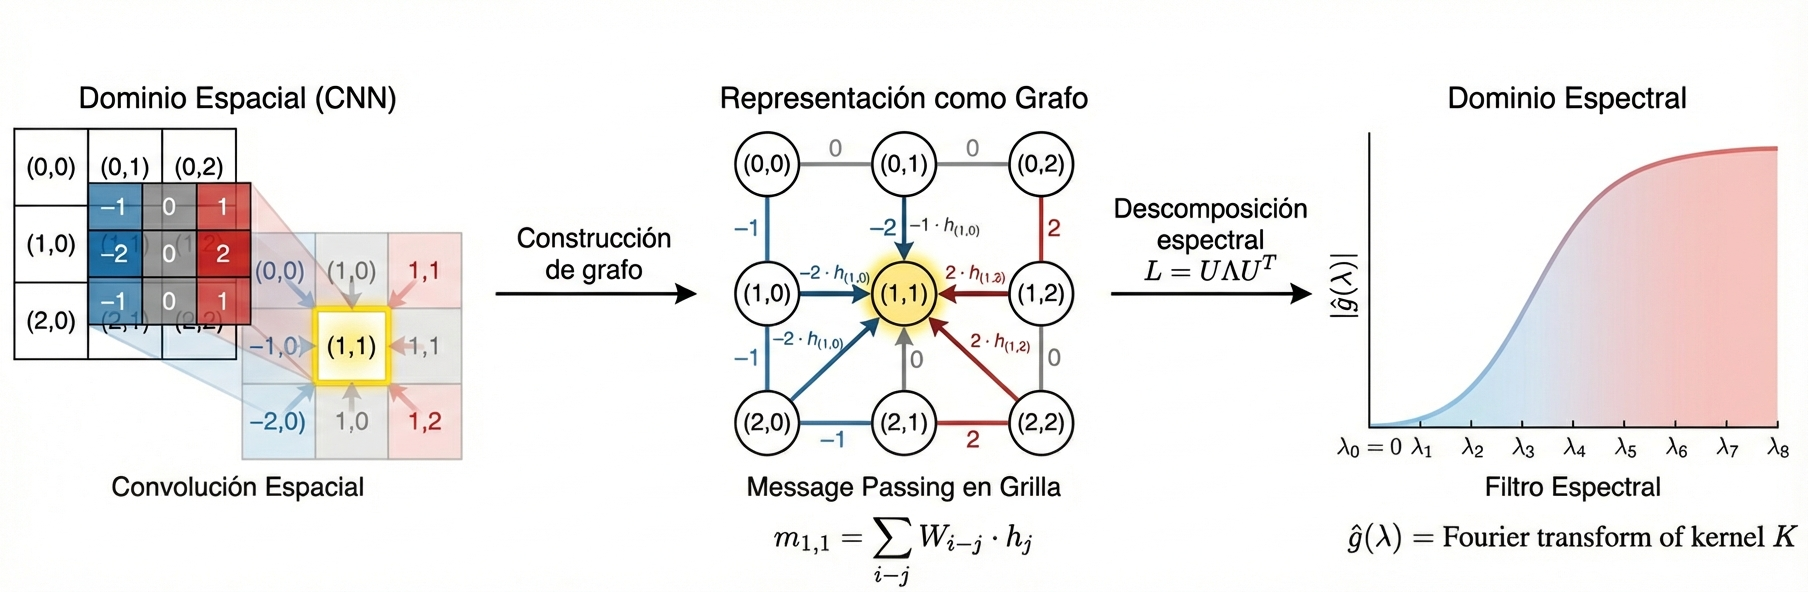
\includegraphics[width=0.85\textwidth]{images/cnn_graph_kernel_spectral}
    \caption[From CNN kernel to spectral representation on graphs]{Transformation of a CNN kernel to a spectral representation on graphs. The spatial kernel of a traditional CNN (left) can be interpreted as a spectral filter over the graph of the regular grid (right), where the eigenvalues of the Laplacian determine the frequencies and the filter modulates each frequency component.}
    \label{fig:cnn_graph_kernel_spectral}
\end{figure}

\begin{theorem}[Spectral Localization]\label{thm:localizacion_espectral}
If a spectral filter $g(\lambda)$ satisfies the decay conditions:
\begin{equation}
|g^{(k)}(\lambda)| \leq C_k (1 + \lambda)^{-k-\epsilon}
\end{equation}
for some $\epsilon > 0$ and constants $C_k$, where $g^{(k)}$ denotes the $k$-th derivative, then $g$ produces operations with local support on the graph.
\end{theorem}

\begin{proof}[Proof sketch]
The filter kernel in the graph domain is $K(i,j) = \sum_k g(\lambda_k) \phi_k(i) \phi_k(j)$, where $\{\lambda_k, \phi_k\}$ are the eigenpairs of the Laplacian. The decay condition on $g^{(k)}$ implies, through generalized integration by parts, that the kernel $K(i,j)$ decays exponentially with the geodesic distance $d(i,j)$ in the graph. Formally, for nodes $i,j$ at distance $d(i,j) > K$ one has $|K(i,j)| \leq C \cdot \alpha^{d(i,j)}$ for some $\alpha < 1$, which guarantees that the filtering operation is essentially local. See \citep[Theorem~5.5]{hammond2011wavelets} for the complete proof in the context of wavelets on graphs.
\end{proof}

\subsubsection{Polynomial Approximation of Filters}

To make spectral convolutions computationally efficient, filters are approximated by polynomials, avoiding the explicit diagonalization of the Laplacian.

\begin{definition}[Polynomial Filters]\label{def:filtros_polinomiales}
A spectral filter $g(\lambda)$ is approximated as:
\begin{equation}
g(\lambda) \approx \sum_{k=0}^K \theta_k p_k(\lambda)
\end{equation}
where $\{p_k\}$ is a polynomial basis and $\{\theta_k\}$ are trainable parameters.
\end{definition}

\begin{example}[Chebyshev Approximation]\label{ex:chebyshev_aproximacion}
Using Chebyshev polynomials $T_k$ on the interval $[-1, 1]$:
\begin{equation}
g(\tilde{\lambda}) = \sum_{k=0}^K \theta_k T_k(\tilde{\lambda})
\end{equation}
where $\tilde{\lambda} = 2\lambda/\lambda_{\max} - 1$ rescales the eigenvalues.
\end{example}

\begin{theorem}[Computational Efficiency]\label{thm:eficiencia_chebyshev}
The Chebyshev approximation allows computing $g(L)f$ in time $O(K|E|)$ without diagonalizing $L$, using the recurrence:
\begin{align}
\bar{x}_0 &= f \\
\bar{x}_1 &= \tilde{L} f \\
\bar{x}_k &= 2\tilde{L}\bar{x}_{k-1} - \bar{x}_{k-2}, \quad k \geq 2
\end{align}
where $\tilde{L} = 2L/\lambda_{\max} - I$.
\end{theorem}

\begin{proof}
By the Chebyshev recurrence, $T_k(\tilde{L})f$ is computed inductively: $\bar{x}_0 = f$ requires $O(n)$, $\bar{x}_1 = \tilde{L}f$ requires a sparse matrix-vector multiplication with cost $O(|E|)$ (since $\tilde{L}$ has at most $2|E| + n$ nonzero entries), and each step $\bar{x}_k = 2\tilde{L}\bar{x}_{k-1} - \bar{x}_{k-2}$ likewise requires $O(|E|)$. Since $K$ recurrence steps are performed, the total cost is $O(K|E|)$. Note that it is not necessary to compute the eigenvalues or eigenvectors of $L$, since the recurrence operates directly with the sparse matrix $\tilde{L}$.
\end{proof}

\subsubsection{Complete Example: Spectral Analysis of a Small Graph}

The following example illustrates all the previous concepts through explicit computations on a 4-node graph.

\begin{example}[Laplacian of a Triangular Graph with an Isolated Vertex]\label{ex:laplaciano_triangulo_4_nodos}
Consider the graph $G$ with 4 vertices and edges $E = \{(1,2), (1,3), (2,3), (3,4)\}$:

\begin{center}
\begin{tikzpicture}[scale=1.2]
    \node[circle, draw, fill=gdlblue!20] (1) at (0, 1) {1};
    \node[circle, draw, fill=gdlblue!20] (2) at (-1, -0.5) {2};
    \node[circle, draw, fill=gdlblue!20] (3) at (1, -0.5) {3};
    \node[circle, draw, fill=gdlgreen!20] (4) at (2.5, 0) {4};

    \draw[thick] (1) -- (2);
    \draw[thick] (1) -- (3);
    \draw[thick] (2) -- (3);
    \draw[thick] (3) -- (4);
\end{tikzpicture}
\end{center}

\textbf{1. Adjacency matrix}:
\begin{equation}
A = \begin{bmatrix}
0 & 1 & 1 & 0 \\
1 & 0 & 1 & 0 \\
1 & 1 & 0 & 1 \\
0 & 0 & 1 & 0
\end{bmatrix}
\end{equation}

\textbf{2. Degree matrix}:
\begin{equation}
D = \begin{bmatrix}
2 & 0 & 0 & 0 \\
0 & 2 & 0 & 0 \\
0 & 0 & 3 & 0 \\
0 & 0 & 0 & 1
\end{bmatrix}
\end{equation}

\textbf{3. Unnormalized Laplacian}:
\begin{equation}
L = D - A = \begin{bmatrix}
2 & -1 & -1 & 0 \\
-1 & 2 & -1 & 0 \\
-1 & -1 & 3 & -1 \\
0 & 0 & -1 & 1
\end{bmatrix}
\end{equation}

\textbf{4. Computation of eigenvalues and eigenvectors}:
The characteristic polynomial is:
\begin{equation}
\det(L - \lambda I) = \lambda(\lambda - 1)(\lambda - 3)(\lambda - 4)
\end{equation}

The eigenvalues are: $\lambda_0 = 0, \lambda_1 = 1, \lambda_2 = 3, \lambda_3 = 4$.

\textbf{Eigenvectors (computed and normalized)}:
\begin{align}
\phi_0 &= \tfrac{1}{2}(1, 1, 1, 1)^T \quad \text{(constant vector, $\lambda_0 = 0$)} \\
\phi_1 &= \tfrac{1}{\sqrt{6}}(-1, -1, 0, 2)^T \quad \text{(smooth variation, $\lambda_1 = 1$)} \\
\phi_2 &= \tfrac{1}{\sqrt{2}}(1, -1, 0, 0)^T \quad \text{(1-2 contrast, $\lambda_2 = 3$)} \\
\phi_3 &= \tfrac{1}{2\sqrt{3}}(1, 1, -3, 1)^T \quad \text{(high frequency, $\lambda_3 = 4$)}
\end{align}

It is verified that $L\phi_k = \lambda_k \phi_k$, $\|\phi_k\| = 1$ and $\langle \phi_i, \phi_j \rangle = \delta_{ij}$ for all $i, j$.

\textbf{5. Frequency interpretation}:
\begin{itemize}
    \item $\phi_0$ (DC): constant function over the entire graph
    \item $\phi_1$ (low frequency): smooth variation, vertex 4 contrasts with vertices 1-2
    \item $\phi_2$ (medium frequency): contrast between vertices 1 and 2
    \item $\phi_3$ (high frequency): rapid oscillation, vertex 3 contrasts strongly with its neighbors
\end{itemize}

\textbf{6. Spectral convolution - Practical example}:
Let $f = (1, 0, -1, 2)^T$ be a signal on the graph and $g(\lambda) = e^{-\lambda/2}$ a low-pass filter.

\textbf{Fourier transform of $f$}:
\begin{align}
\hat{f}_0 &= \phi_0^T f = \tfrac{1}{2}(1 + 0 - 1 + 2) = 1 \\
\hat{f}_1 &= \phi_1^T f = \tfrac{1}{\sqrt{6}}(-1 + 0 + 0 + 4) = \tfrac{3}{\sqrt{6}} = \tfrac{\sqrt{6}}{2} \\
\hat{f}_2 &= \phi_2^T f = \tfrac{1}{\sqrt{2}}(1 - 0 + 0 + 0) = \tfrac{1}{\sqrt{2}} = \tfrac{\sqrt{2}}{2} \\
\hat{f}_3 &= \phi_3^T f = \tfrac{1}{2\sqrt{3}}(1 + 0 + 3 + 2) = \tfrac{6}{2\sqrt{3}} = \sqrt{3}
\end{align}

\textbf{Filter application}:
\begin{align}
g(\lambda_0) \hat{f}_0 &= e^{0} \cdot 1 = 1 \\
g(\lambda_1) \hat{f}_1 &= e^{-1/2} \cdot \tfrac{\sqrt{6}}{2} \approx 0.74 \\
g(\lambda_2) \hat{f}_2 &= e^{-3/2} \cdot \tfrac{\sqrt{2}}{2} \approx 0.16 \\
g(\lambda_3) \hat{f}_3 &= e^{-2} \cdot \sqrt{3} \approx 0.23
\end{align}

\textbf{Filtered signal}:
\begin{equation}
f_{\text{filtered}} = \sum_{k=0}^{3} g(\lambda_k)\hat{f}_k \phi_k \approx (0.38, 0.15, 0.30, 1.17)^T
\end{equation}

\textbf{Interpretation}: The low-pass filter has smoothed the signal, especially reducing the high-frequency components ($\lambda_2 = 3$ and $\lambda_3 = 4$) while preserving the constant component.
\end{example}

\textbf{Computational Implementation of the Example.} The computational verification of the example follows this methodology:

\textbf{Graph construction}:
\begin{enumerate}
    \item Define 4 nodes with specific connectivity: $(1,2)$, $(1,3)$, $(2,3)$, $(3,4)$
    \item Compute adjacency and Laplacian matrices using standard libraries
    \item Verify basic properties: symmetry, positive semi-definiteness
\end{enumerate}

\textbf{Spectral analysis}:
\begin{itemize}
    \item \textbf{Eigenvalues}: $\{0, 1, 3, 4\}$ with clear frequency interpretation
    \item \textbf{Eigenvectors}: Orthogonal basis for representing signals on the graph
    \item \textbf{Verification}: Check orthogonality and normalization properties
\end{itemize}

\textbf{Spectral convolution}:
For the test signal $f = [1, 0, -1, 2]^T$ and low-pass filter $g(\lambda) = e^{-\lambda/2}$:
\begin{enumerate}
    \item \textbf{Forward transform}: $\hat{f} = U^T f$ using eigenvectors
    \item \textbf{Filtering}: Multiplication by $g(\lambda_k)$ for each component
    \item \textbf{Inverse transform}: $f_{filtered} = U \hat{f}_{filtered}$
\end{enumerate}

\textbf{Numerical results}:
The low-pass filter produces a smoothed signal $\approx [0.38, 0.15, 0.30, 1.17]^T$, demonstrating the attenuation of high-frequency components while preserving the global trends.

\textbf{Observations from the Example.} This example illustrates key concepts of spectral analysis on graphs:

\textbf{1. Connectivity and multiplicity}:
The graph is connected, so $\lambda_0 = 0$ has multiplicity 1.

\textbf{2. Geometric interpretation}:
- The low-frequency eigenvectors capture the global structure
- The high-frequency ones reveal local variations between adjacent nodes

\textbf{3. Effective filtering}:
The low-pass filter $e^{-\lambda/2}$ preserves the DC component and progressively attenuates the higher frequencies.

\textbf{4. Computational complexity}:
- Diagonalization: $O(n^3)$ for $n = 4$ (trivial)
- For large graphs, the Chebyshev polynomial approximation is preferred

\begin{example}[Other Types of Spectral Filters]\label{ex:otros_filtros_espectrales}
\leavevmode
\begin{enumerate}
    \item \textbf{Rational Filters}: $g(\lambda) = \frac{P(\lambda)}{Q(\lambda)}$ where $P, Q$ are polynomials
    \item \textbf{Lanczos Filters}: $g(\lambda) = \theta \cdot \operatorname{sinc}(\pi\lambda/\lambda_{\max})$
    \item \textbf{Splines}: Piecewise spline functions over the spectrum
    \item \textbf{Wavelet Filters}: Based on spectral wavelets on graphs
\end{enumerate}
\end{example}

\textbf{Localization vs Efficiency Trade-off.} There is a fundamental trade-off:
\begin{itemize}
    \item \textbf{Global spectral filters}: More expressive but $O(n^3)$ for diagonalization
    \item \textbf{Polynomial approximations}: Local and efficient $O(K|E|)$ but less expressive
    \item \textbf{Polynomial degree $K$}: Controls the radius of spatial localization
\end{itemize}

\subsection{Wavelet Bases and Multiresolution Analysis}\label{subsec:wavelets_multirresolucion}

Wavelets provide an alternative to the Fourier transform that allows simultaneous time-frequency analysis, overcoming the limitations of the uncertainty principle. Their application in neural networks offers natural hierarchical representations.

\begin{definition}[Mother Wavelet]\label{def:wavelet_madre}
A function $\psi \in L^2(\mathbb{R})$ is a \textbf{mother wavelet} if it satisfies the admissibility condition:
\begin{equation}
C_\psi = \int_{-\infty}^{\infty} \frac{|\hat{\psi}(\omega)|^2}{|\omega|} d\omega < \infty
\end{equation}
where $\hat{\psi}$ is the Fourier transform of $\psi$.
\end{definition}

\textbf{Implications of the Admissibility Condition.} The condition $C_\psi < \infty$ implies that $\hat{\psi}(0) = 0$, which means $\int_{-\infty}^{\infty} \psi(t) dt = 0$. This guarantees that wavelets have zero mean and provide local analysis.

\begin{definition}[Continuous Wavelet Transform]\label{def:transformada_wavelet_continua}
For a function $f \in L^2(\mathbb{R})$ and mother wavelet $\psi$, the continuous wavelet transform is defined as:
\begin{equation}
W_f(a, b) = \frac{1}{\sqrt{|a|}} \int_{-\infty}^{\infty} f(t) \psi^*\left(\frac{t-b}{a}\right) dt
\end{equation}
where $a \in \mathbb{R}\setminus\{0\}$ is the scale parameter and $b \in \mathbb{R}$ is the translation parameter.
\end{definition}

\begin{theorem}[Wavelet Reconstruction Formula]\label{thm:reconstruccion_wavelet}
If $\psi$ satisfies the admissibility condition, then:
\begin{equation}
f(t) = \frac{1}{C_\psi} \int_{-\infty}^{\infty} \int_{-\infty}^{\infty} W_f(a, b) \psi_{a,b}(t) \frac{da \, db}{a^2}
\end{equation}
where $\psi_{a,b}(t) = \frac{1}{\sqrt{|a|}} \psi\left(\frac{t-b}{a}\right)$.

See Section~\ref{sec:reconstruccion_wavelet} of \autoref{ch:teoremas_complementarios} for the complete proof.
\end{theorem}

\begin{definition}[Multiresolution Analysis (MRA)]\label{def:mra}
A \textbf{multiresolution analysis} of $L^2(\mathbb{R})$ is a sequence of closed subspaces $\{V_j\}_{j \in \mathbb{Z}}$ that satisfies:
\begin{enumerate}
    \item \textbf{Inclusion}: $\cdots \subset V_{-1} \subset V_0 \subset V_1 \subset \cdots$
    \item \textbf{Density}: $\overline{\bigcup_{j \in \mathbb{Z}} V_j} = L^2(\mathbb{R})$
    \item \textbf{Separation}: $\bigcap_{j \in \mathbb{Z}} V_j = \{0\}$
    \item \textbf{Scaling}: $f(x) \in V_j \Leftrightarrow f(2x) \in V_{j+1}$
    \item \textbf{Translation}: $f(x) \in V_0 \Rightarrow f(x-k) \in V_0$ for $k \in \mathbb{Z}$
    \item \textbf{Riesz basis}: There exists $\phi \in V_0$ such that $\{\phi(x-k)\}_{k \in \mathbb{Z}}$ is a Riesz basis of $V_0$
\end{enumerate}
\end{definition}

\begin{definition}[Scaling Function]\label{def:funcion_escala}
The function $\phi$ in condition 6 of the MRA is called the \textbf{scaling function} or \textbf{father wavelet}. It satisfies the scaling equation:
\begin{equation}
\phi(x) = \sqrt{2} \sum_{k \in \mathbb{Z}} h_k \phi(2x - k)
\end{equation}
where $\{h_k\}$ are the scaling coefficients.
\end{definition}

\begin{definition}[Orthogonal Wavelet]\label{def:wavelet_ortogonal}
Given an MRA with scaling function $\phi$, the associated \textbf{orthogonal wavelet} is defined as:
\begin{equation}
\psi(x) = \sqrt{2} \sum_{k \in \mathbb{Z}} g_k \phi(2x - k)
\end{equation}
where $g_k = (-1)^k h_{1-k}$ are related to the scaling coefficients.
\end{definition}

\begin{theorem}[Wavelet Decomposition]\label{thm:descomposicion_wavelet}
Every function $f \in L^2(\mathbb{R})$ can be decomposed as:
\begin{equation}
f(x) = \sum_{k \in \mathbb{Z}} c_{J,k} \phi_{J,k}(x) + \sum_{j=J}^{\infty} \sum_{k \in \mathbb{Z}} d_{j,k} \psi_{j,k}(x)
\end{equation}
where $\phi_{j,k}(x) = 2^{j/2} \phi(2^j x - k)$ and $\psi_{j,k}(x) = 2^{j/2} \psi(2^j x - k)$.

See Section~\ref{sec:descomposicion_wavelet} of \autoref{ch:teoremas_complementarios} for the proof.
\end{theorem}

\begin{example}[Haar Wavelets]\label{ex:wavelets_haar}
The Haar wavelets are the simplest:
\begin{align}
\phi(x) &= \begin{cases} 1 & \text{if } 0 \leq x < 1 \\ 0 & \text{otherwise} \end{cases} \\
\psi(x) &= \begin{cases} 1 & \text{if } 0 \leq x < 1/2 \\ -1 & \text{if } 1/2 \leq x < 1 \\ 0 & \text{otherwise} \end{cases}
\end{align}
\end{example}

\begin{example}[Daubechies Wavelets]\label{ex:wavelets_daubechies}
The Daubechies wavelets $D_N$ have compact support $[0, 2N-1]$ and $N$ vanishing moments:
\begin{equation}
\int_{-\infty}^{\infty} x^k \psi(x) dx = 0, \quad k = 0, 1, \ldots, N-1
\end{equation}
\end{example}

\subsubsection{Wavelets on Graphs}

\begin{definition}[Spectral Wavelets on Graphs]\label{def:wavelets_grafos}
For a graph with Laplacian $L$ and eigenvectors $\{\phi_k\}$, the spectral wavelets are defined as:
\begin{equation}
\psi_{s,i} = \sum_{k=0}^{n-1} g(s\lambda_k) \phi_k(i) \phi_k
\end{equation}
where $g$ is a mother wavelet function and $s$ is the scale parameter.
\end{definition}

\begin{example}[GraphWavelets]\label{ex:graph_wavelets}
A common choice for the mother function is:
\begin{equation}
g(x) = x e^{-x}
\end{equation}
which provides both spectral and spatial localization on the graph.
\end{example}

\textbf{Advantages of Wavelets in CNNs.} Wavelets offer specific advantages for neural networks:
\begin{itemize}
    \item \textbf{Multiresolution analysis}: Natural for hierarchical architectures
    \item \textbf{Localization}: Better than Fourier for local features
    \item \textbf{Parsimony}: Sparse representations for natural signals
    \item \textbf{Translation invariance}: Approximate depending on the type of wavelet
\end{itemize}

\subsubsection{Morlet Wavelet and Time-Frequency Analysis}

\begin{definition}[Morlet Wavelet]\label{def:wavelet_morlet}
The \textit{Morlet wavelet} is a wave modulated by a Gaussian:
\begin{equation}
\psi_{\omega_0}(t) = c_\sigma \pi^{-1/4} e^{i\omega_0 t} e^{-t^2/2}
\end{equation}
where $\omega_0 \geq 5$ is the central frequency and $c_\sigma$ is a normalization constant. Its Fourier transform is $\hat{\psi}_{\omega_0}(\omega) = c_\sigma \pi^{-1/4} e^{-(\omega - \omega_0)^2/2}$, a Gaussian centered at $\omega_0$.
\end{definition}

\begin{remark}[Optimal Time-Frequency Resolution]
The Morlet wavelet achieves equality in the Heisenberg-Gabor uncertainty principle:
\[
\Delta t \cdot \Delta \omega = \frac{1}{2}
\]
which makes it the wavelet with the best simultaneous resolution in time and frequency. At scale $a$, the wavelet $\psi_{a,b}(t) = a^{-1/2}\psi((t-b)/a)$ has temporal resolution $\Delta t \propto a$ and frequency resolution $\Delta \omega \propto 1/a$, exactly implementing the adaptive multiresolution property.
\end{remark}

\subsubsection{Scattering Transform: CNNs with Predefined Wavelets}

The deepest connection between wavelets and CNNs is established through Mallat's \textit{Scattering Transform}~\citep{Mallat2012scattering}, which shows that the early layers of a CNN can be understood as a bank of wavelet filters with a modulus nonlinearity.

\begin{definition}[Scattering Transform]\label{def:scattering_transform}
Let $\psi$ be a mother wavelet and $\phi$ a scaling function (low-pass). The \textit{scattering operator} of order $m$ is defined recursively:
\begin{align}
S_0 f &= f \star \phi_J \\
S_1 f &= \{|f \star \psi_{j_1}| \star \phi_J\}_{j_1} \\
S_m f &= \{|\cdots|f \star \psi_{j_1}| \star \psi_{j_2}| \cdots \star \psi_{j_m}| \star \phi_J\}_{j_1 < j_2 < \cdots < j_m}
\end{align}
where $\psi_j(t) = 2^{-j}\psi(2^{-j}t)$ are the dilated wavelets and $\phi_J$ is the scaling function at the coarsest resolution.
\end{definition}

\begin{proposition}[Properties of the Scattering Transform]\label{prop:propiedades_scattering}
The scattering operator $Sf = (S_0 f, S_1 f, S_2 f, \ldots)$ satisfies:
\begin{enumerate}
    \item \textbf{Translation invariance}: $S[\tau_c f] = S[f]$ for every translation $\tau_c f(t) = f(t - c)$.
    \item \textbf{Lipschitz stability to deformations}: For every diffeomorphism $\tau$ close to the identity:
    \begin{equation}
    \|Sf - S(f \circ \tau)\| \leq C\|\nabla \tau\|_\infty \|f\|
    \end{equation}
    \item \textbf{Energy conservation}: $\sum_{m=0}^{\infty} \|S_m f\|^2 = \|f\|^2$.
\end{enumerate}
\end{proposition}

\begin{proof}
(1) Translation commutes with convolution: $\tau_c f \star \psi_j = \tau_c(f \star \psi_j)$. The modulus preserves this translation: $|\tau_c(f \star \psi_j)| = \tau_c|f \star \psi_j|$. Finally, convolution with $\phi_J$ (low-pass at scale $2^J$) averages over translations smaller than $2^J$, eliminating the dependence on $c$.

(2) Since $\psi_j$ has frequency support concentrated at $|\omega| \sim 2^j$, the convolution $f \star \psi_j$ is sensitive to variations of $f$ at scale $2^{-j}$. A deformation $\tau$ with $\|\nabla \tau\|_\infty \leq \epsilon$ shifts the frequencies by at most $\epsilon \cdot 2^j$, which is small compared to the bandwidth $2^j$ of the filter, producing an error proportional to $\epsilon$.

(3) It follows from Parseval's identity for wavelets: $\|f\|^2 = \|f \star \phi_J\|^2 + \sum_j \|f \star \psi_j\|^2$. Applying this iteratively to the coefficients $|f \star \psi_j|$ and using that the modulus preserves the $L^2$ norm, total energy conservation is obtained.
\end{proof}

\begin{remark}[Scattering as a CNN with Fixed Weights]
The architecture of the scattering transform is isomorphic to a CNN with the following correspondences:
\begin{itemize}
    \item \textbf{Filters}: Predefined (not learned) wavelets $\psi_j$ $\leftrightarrow$ convolutional kernels
    \item \textbf{Nonlinearity}: Modulus $|{\cdot}|$ $\leftrightarrow$ ReLU
    \item \textbf{Pooling}: Convolution with $\phi_J$ $\leftrightarrow$ average pooling
    \item \textbf{Depth}: Scattering order $m$ $\leftrightarrow$ number of layers
\end{itemize}
The key difference is that the scattering transform has theoretical guarantees of stability and invariance, while trained CNNs learn them implicitly.
\end{remark}

\begin{figure}[htbp]
	\centering
	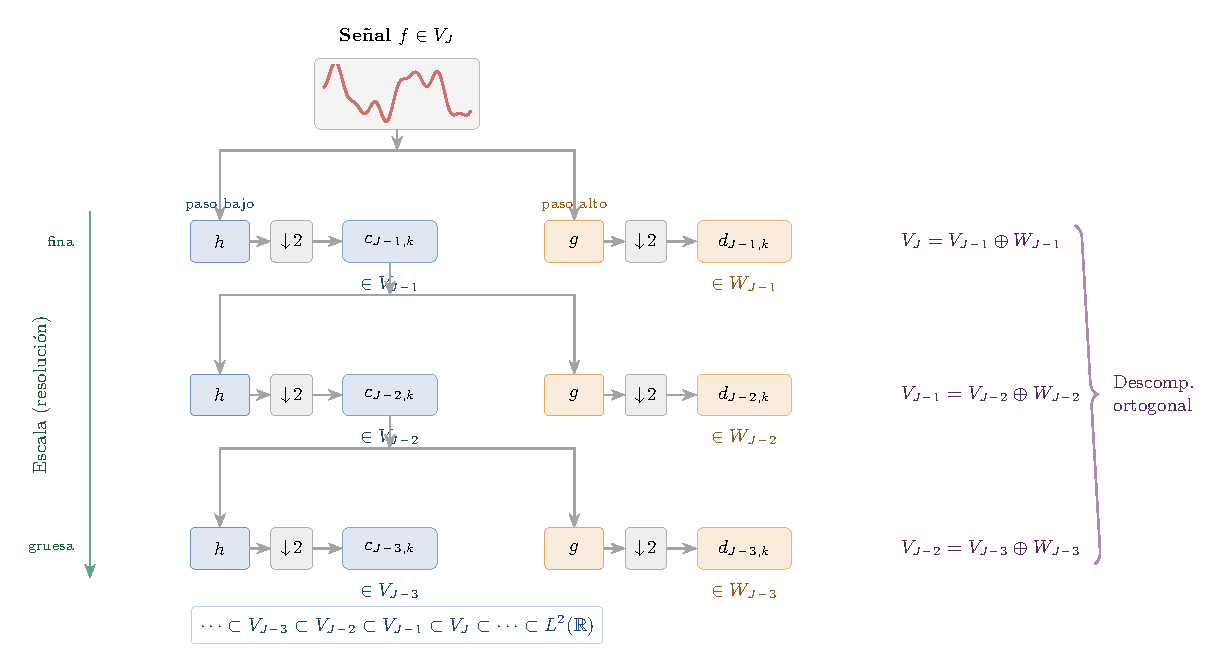
\includegraphics[width=0.85\textwidth]{images/wavelet_multiresolution}
	\caption[Multiresolution wavelet decomposition]{Multiresolution wavelet decomposition: a signal is iteratively decomposed through low-pass ($h$) and high-pass ($g$) filters followed by downsampling ($\downarrow 2$), separating the approximation ($c_{j,k}$) and detail ($d_{j,k}$) components at multiple scales.}
	\label{fig:wavelet_multiresolution}
\end{figure}

\subsection{Spectral Convolutions in CNNs}\label{subsec:convoluciones_espectrales_cnns}

Spectral convolutions in CNNs leverage the properties of the frequency domain to implement convolutional operations efficiently, especially for large kernels or in applications with specific geometric structure.

\begin{definition}[Parametrized Spectral Filter]\label{def:filtro_espectral_parametrizado}
A \textbf{parametrized spectral filter} is a function $h_\theta: \mathbb{R}_+ \to \mathbb{R}$ where $\theta \in \mathbb{R}^p$ are trainable parameters. The filter acts on the frequency spectrum through:
\begin{equation}
h_\theta(\lambda) = \sum_{k=0}^{K-1} \theta_k \phi_k(\lambda)
\end{equation}
where $\{\phi_k\}$ is a basis of functions (polynomials, wavelets, etc.).
\end{definition}

\begin{definition}[Spectral Convolutional Layer]\label{def:capa_convolucional_espectral}
A spectral convolutional layer transforms an input signal $x \in \mathbb{R}^n$ through:
\begin{equation}
y = \sigma(h_\theta \star x + b)
\end{equation}
where:
\begin{itemize}
    \item $h_\theta \star x$ is the spectral convolution: $\mathcal{F}^{-1}[h_\theta(\cdot) \cdot \mathcal{F}[x]]$
    \item $\sigma$ is the activation function
    \item $b$ is the bias term
\end{itemize}
\end{definition}

\begin{theorem}[Spatial-Spectral Equivalence]\label{thm:equivalencia_espacial_espectral}
For domains with regular structure (grids, tori), spatial and spectral convolutions are mathematically equivalent:
\begin{equation}
(f * g)(x) = \mathcal{F}^{-1}[\mathcal{F}[f] \cdot \mathcal{F}[g]](x)
\end{equation}
However, they differ in:
\begin{itemize}
    \item \textbf{Computational complexity}: Spatial $O(n \cdot k^2)$ vs Spectral $O(n \log n)$
    \item \textbf{Localization}: Spatial (local) vs Spectral (global)
    \item \textbf{Interpretability}: Spatial (geometric) vs Spectral (frequency)
\end{itemize}
\end{theorem}

\begin{proof}
The equivalence follows from the convolution theorem for the Fourier transform. For functions $f, g \in L^1(\mathbb{R}^d)$ (or their discrete analogs on $\mathbb{Z}^d$), the Fourier transform satisfies $\mathcal{F}[f * g] = \mathcal{F}[f] \cdot \mathcal{F}[g]$. Applying $\mathcal{F}^{-1}$ to both sides yields the identity of the statement. The differences in complexity are: the direct spatial convolution performs $O(n \cdot k^2)$ operations (traversing $n$ positions applying a kernel of size $k \times k$), while the spectral convolution via FFT requires $O(n \log n)$ for the forward transform, $O(n)$ for the pointwise multiplication, and $O(n \log n)$ for the inverse transform, totaling $O(n \log n)$. The localization differs because a finite spatial kernel of size $k$ corresponds to a spectral filter with full support, and vice versa.
\end{proof}

\subsubsection{Practical Implementation of Spectral CNNs}

\textbf{Algorithm: Spectral Forward Pass.}\label{alg:forward_espectral} For an input $x \in \mathbb{R}^{H \times W}$ and parametrized filter $h_\theta$:
\begin{enumerate}
    \item \textbf{Forward transform}: $\hat{x} = \text{FFT2D}(x)$
    \item \textbf{Filter application}: $\hat{y} = h_\theta(\omega) \odot \hat{x}$ (element-wise product)
    \item \textbf{Inverse transform}: $y = \text{IFFT2D}(\hat{y})$
    \item \textbf{Activation}: $z = \sigma(y + b)$
\end{enumerate}

\textbf{Implementation Considerations.}
\begin{itemize}
    \item \textbf{Padding}: To avoid edge effects, circular padding or zero-padding is used
    \item \textbf{Numerical precision}: \gls{FFT}/IFFT can accumulate floating-point errors
    \item \textbf{Memory}: Store both the spatial and spectral representations
\end{itemize}

\begin{definition}[Transfer Function of a Linear CNN]\label{def:funcion_transferencia_cnn}
For a linear CNN (without nonlinear activation functions) with $L$ layers, the global transfer function in the frequency domain is:
\begin{equation}
H(\omega) = \prod_{l=1}^L H_l(\omega)
\end{equation}
where $H_l(\omega)$ is the frequency response of layer $l$. This factorization is only valid in the absence of nonlinearities between layers.
\end{definition}

\begin{example}[Simple Spectral CNN]\label{ex:cnn_espectral_simple}
Consider a two-layer CNN:
\begin{align}
\text{Layer 1}: \quad y_1 &= \sigma(\mathcal{F}^{-1}[h_1(\omega) \cdot \mathcal{F}[x]] + b_1) \\
\text{Layer 2}: \quad y_2 &= \mathcal{F}^{-1}[h_2(\omega) \cdot \mathcal{F}[y_1]] + b_2
\end{align}
The total frequency response is $H(\omega) = h_1(\omega) \cdot h_2(\omega)$ (without considering nonlinearities).
\end{example}

\subsubsection{Complexity Analysis}

\begin{theorem}[Computational Complexity]\label{thm:complejidad_convoluciones_espectrales}
For a 2D convolution of size $n \times n$ with a $k \times k$ kernel:
\begin{itemize}
    \item \textbf{Direct convolution}: $O(n^2 k^2)$
    \item \textbf{Spectral convolution}: $O(n^2 \log n)$
    \item \textbf{Break-even point}: Spectral is more efficient when $k > O(\log n)$
\end{itemize}
\end{theorem}

\begin{proof}
The direct 2D convolution computes, for each of the $n^2$ positions of the image, a sum of $k^2$ products, giving $O(n^2 k^2)$ operations. The spectral convolution requires: (i) 2D FFT of the image: $O(n^2 \log n)$; (ii) 2D FFT of the kernel (with zero-padding): $O(n^2 \log n)$; (iii) pointwise multiplication in frequency: $O(n^2)$; (iv) 2D IFFT: $O(n^2 \log n)$. The total is $O(n^2 \log n)$. The break-even point is obtained by equating $n^2 k^2 = n^2 \log n$, that is, $k^2 = \log n$, so the spectral convolution is preferable when $k > O(\sqrt{\log n})$.
\end{proof}

\begin{example}[Practical Efficiency Analysis]\label{ex:eficiencia_practica}
For a $512 \times 512$ image and a $k \times k$ kernel:
\begin{itemize}
    \item $k = 3$: Direct: $\sim 2.3 \times 10^6$ ops, Spectral: $\sim 2.6 \times 10^6$ ops
    \item $k = 15$: Direct: $\sim 5.9 \times 10^7$ ops, Spectral: $\sim 2.6 \times 10^6$ ops
    \item $k = 51$: Direct: $\sim 6.8 \times 10^8$ ops, Spectral: $\sim 2.6 \times 10^6$ ops
\end{itemize}
\end{example}

\begin{theorem}[Spectral Universal Approximation]\label{thm:aproximacion_universal_espectral}
Let $\mathcal{G} = (V, E)$ be a finite graph with Laplacian $L$ and spectrum contained in $[0, \lambda_{\max}]$. For any continuous spectral filter $h: [0, \lambda_{\max}] \to \mathbb{R}$ and $\epsilon > 0$, there exists a polynomial filter $p(\lambda) = \sum_{k=0}^{K} \theta_k T_k(\tilde{\lambda})$ of sufficiently large degree $K$ such that:
\begin{equation}
\|h(\lambda) - p(\lambda)\|_{\infty, [0, \lambda_{\max}]} < \epsilon
\end{equation}
Consequently, the filtered signal satisfies $\|h(L)f - p(L)f\| \leq \epsilon \|f\|$ for every signal $f$ on the graph.
\end{theorem}

\begin{proof}[Sketch]
The spectral interval $[0, \lambda_{\max}]$ is compact, so the result is a direct consequence of the Weierstrass approximation theorem: every continuous function on a compact interval can be uniformly approximated by polynomials. The bound on the filtered signal follows from $\|h(L)f - p(L)f\| = \|(h-p)(L)f\| \leq \|h - p\|_\infty \|f\|$, since the eigenvalues of $(h-p)(L)$ are bounded by $\|h-p\|_\infty$.
\end{proof}

\textbf{Limitations of Spectral Convolutions.}
\begin{itemize}
    \item \textbf{Non-locality}: Spectral filters affect the signal globally
    \item \textbf{Regularity}: They require domains with \gls{FFT} structure (regular grids)
    \item \textbf{Boundaries}: Difficulties with non-periodic boundary conditions
    \item \textbf{Interpretability}: Less intuitive than spatial convolution
\end{itemize}

\subsection{Frequency Interpretation of Classical CNNs}\label{subsec:interpretacion_frecuencial_cnns}

The frequency analysis of traditional CNNs reveals deep insights into what features they learn and how they process visual information.

\begin{definition}[Frequency Response of a Kernel]\label{def:respuesta_frecuencial_kernel}
For a convolutional kernel $K \in \mathbb{R}^{k \times k}$, its frequency response is:
\begin{equation}
H(\omega_x, \omega_y) = \sum_{i=0}^{k-1} \sum_{j=0}^{k-1} K[i,j] e^{-2\pi i(\omega_x i + \omega_y j)}
\end{equation}
\end{definition}

\begin{example}[Analysis of Common Kernels]\label{ex:analisis_kernels_comunes}
\textbf{1. Sobel Edge Detector}:
\begin{equation}
K_{\text{Sobel}} = \begin{bmatrix} -1 & 0 & 1 \\ -2 & 0 & 2 \\ -1 & 0 & 1 \end{bmatrix}
\end{equation}
Frequency response: high-pass with maximum at medium horizontal frequencies.

\textbf{2. Gaussian Filter}:
\begin{equation}
K_{\text{Gauss}}[i,j] = \frac{1}{2\pi\sigma^2} e^{-\frac{(i-c)^2 + (j-c)^2}{2\sigma^2}}
\end{equation}
Frequency response: low-pass with a smooth cutoff determined by $\sigma$.

\textbf{3. Laplacian}:
\begin{equation}
K_{\text{Lap}} = \begin{bmatrix} 0 & -1 & 0 \\ -1 & 4 & -1 \\ 0 & -1 & 0 \end{bmatrix}
\end{equation}
Frequency response: isotropic high-pass.
\end{example}

\begin{remark}[Spectral Evolution during Training]\label{rem:evolucion_espectral}
Empirical observations show that, during the training of a CNN, the spectral distribution of the filters evolves following a characteristic pattern:
\begin{enumerate}
    \item \textbf{Early layers}: Low-pass filters and edge detectors (high frequencies)
    \item \textbf{Intermediate layers}: Band-pass filters for specific textures
    \item \textbf{Deep layers}: Complex filters, less spectrally interpretable
\end{enumerate}
This behavior has been documented experimentally in multiple architectures, although it lacks a general formal proof.
\end{remark}

\textbf{Experiment: Spectral Bias of CNNs.}\label{exp:sesgo_espectral} Empirical studies show that CNNs exhibit a bias toward low frequencies:
\begin{itemize}
    \item They first learn low-frequency components
    \item They require more iterations to capture high-frequency details
    \item This bias can be improved with spectral initialization techniques
\end{itemize}

The spectral methods developed in this section find direct applications in domains where the frequency structure of the data is fundamental: medical image reconstruction (MRI, computed tomography), scientific signal processing (astronomy, seismology), and neural network compression through spectral pruning. The focus of this thesis, however, is centered on the mathematical foundation of these methods.

\subsection{Limitations and Challenges}\label{subsec:aplicaciones_limitaciones}

\textbf{Limitation: Dependence on the Domain Geometry.}\label{lim:geometria_dominio} Classical spectral convolutions require:
\begin{itemize}
    \item \textbf{Regular structure}: Uniform grids for efficient \gls{FFT}
    \item \textbf{Boundary conditions}: Periodic or with adequate padding
    \item \textbf{Fixed size}: Difficulties with variable-size data
\end{itemize}

\textbf{Consequence}: Restriction to regular Euclidean domains.

\textbf{Limitation: Localization-Efficiency Trade-off.}\label{lim:tradeoff_localizacion}
\begin{table}[h]
\centering
\begin{tabular}{|l|c|c|c|}
\hline
\textbf{Method} & \textbf{Localization} & \textbf{Efficiency} & \textbf{Interpretability} \\
\hline
Spatial convolution & Excellent & Medium & High \\
Spectral convolution & Poor & Excellent & Medium \\
Polynomial approximation & Good & Good & Medium \\
Wavelets & Excellent & Medium & High \\
\hline
\end{tabular}
\caption{Comparison of convolutional methods}
\label{tab:comparacion_metodos}
\end{table}

\textbf{Limitation: Numerical Stability.}\label{lim:estabilidad_numerica} Spectral methods can suffer from:
\begin{itemize}
    \item \textbf{Error accumulation}: In multiple \gls{FFT}/IFFT
    \item \textbf{Aliasing}: In downsampling without anti-aliasing filters
    \item \textbf{Floating-point precision}: Especially on GPU
\end{itemize}

\textbf{Limitation: Reduced Interpretability.}\label{lim:interpretabilidad} Compared to spatial convolutions:
\begin{itemize}
    \item Spectral filters are less visually intuitive
    \item The relationship with geometric features is indirect
    \item Debugging and error analysis are more complex
\end{itemize}

\textbf{Limitation: No Spectral Transferability between Domains.}\label{lim:transferibilidad} Spectral filters defined over a domain $\Omega_1$ cannot be directly transferred to another domain $\Omega_2$ with a different spectrum. Formally, if $\{\lambda_k^{(1)}, \phi_k^{(1)}\}$ and $\{\lambda_k^{(2)}, \phi_k^{(2)}\}$ are the spectral decompositions of the Laplacian operators on $\Omega_1$ and $\Omega_2$ respectively, a filter $h(\lambda)$ learned over $\{\lambda_k^{(1)}\}$ has no canonical interpretation over $\{\lambda_k^{(2)}\}$ unless there exists a natural correspondence between the eigenvalues. This limitation motivates the use of polynomial approximations such as Chebyshev filters (\autoref{thm:localizacion_espectral}), which define the filter as a function of the operator $h(L)$ instead of acting on individual eigenvalues.

\begin{proposition}[Fundamental Localization-Globality Trade-off]\label{prop:tradeoff_localizacion}
Let $h(\lambda)$ be a spectral filter with support in $[\lambda_{\min}, \lambda_{\max}]$ and let $K(x,y) = \sum_k h(\lambda_k) \phi_k(x)\phi_k(y)$ be its associated spatial kernel. Then:
\begin{equation}
\text{supp}_{\text{freq}}(h) \cdot \text{supp}_{\text{spatial}}(K) \geq C > 0
\end{equation}
where $C$ depends only on the dimension of the domain. In particular, a filter perfectly localized in frequency ($h = \delta_{\lambda_k}$) is completely delocalized in space ($K(x,y) = \phi_k(x)\phi_k(y)$, global support).
\end{proposition}

\begin{proof}
It is a direct consequence of the uncertainty principle for the spectral transform: the concentration of a function and its spectral representation cannot both be arbitrarily small simultaneously. For the case $h = \delta_{\lambda_k}$, the kernel reduces to $K(x,y) = \phi_k(x)\phi_k(y)$, which is nonzero over almost the entire domain (since the eigenvectors of the Laplacian vanish only on a set of measure zero). The general case follows by a duality argument analogous to the classical Heisenberg principle.
\end{proof}

\textbf{Synthesis: The Spectral Perspective as a Bridge.} Harmonic analysis provides a unifying framework that connects:
\begin{enumerate}
    \item \textbf{Classical CNNs} (Fourier analysis on regular grids)
    \item \textbf{Spectral GCNs} (spectral analysis on graphs)
    \item \textbf{Geometric CNNs} (harmonic analysis on groups and manifolds)
    \item \textbf{Transformers} (attention as adaptive convolution in the frequency domain)
\end{enumerate}

This perspective reveals that many seemingly different architectures share deep mathematical foundations, facilitating the development of new architectures that combine the best features of each approach.

The \gls{analisis_armonico} developed in the preceding section not only enriches our understanding of classical CNNs, but also provides the mathematical tools needed to establish the fundamental equivalence between convolutions on regular grids and spectral operations on graphs. This connection, which we will explore next, constitutes one of the pillars of the unifying framework of Geometric Deep Learning.

\section[From Convolutions to Graphs: CNN-GNN Connection]{From Convolutions to Graphs: \glspl{CNN}-\glspl{GNN} Connection}\label{sec:cnn_as_gnn}

\subsection{Preliminaries: Graph Theory}\label{subsec:preliminares_grafos_cnn}
